%
% \iffalse meta-comment
%
% Copyright 2016 Brian Dunn
%
% This work may be distributed and/or modified under the
% conditions of the LaTeX Project Public License, either version 1.3
% of this license or (at your option) any later version.
% The latest version of this license is in
%   http://www.latex-project.org/lppl.txt
% and version 1.3 or later is part of all distributions of LaTeX
% version 2005/12/01 or later.
%
% \fi

%
% \iffalse
%<package>\NeedsTeXFormat{LaTeX2e}
%<package>\ProvidesPackage{keyfloat}
%<package>    [2017/05/12 v0.15 Key/value interface for floats and the subcaption package.]
%
%<*driver>
\documentclass{ltxdoc}

\newcommand*{\mypackagename}{keyfloat}
\newcommand{\quicksummary}{Provides a key/value interface for generating floats.}


\usepackage{lmodern}
% \usepackage{libertine}
\usepackage[T1]{fontenc}
\usepackage[utf8]{inputenc}
\usepackage{textcomp}	% provides \degree, \textquotesingle, \textmu


\newcommand*{\TakeFourierOrnament}[1]{{%
\fontencoding{U}\fontfamily{futs}\selectfont\char#1}}

\newcommand*{\textwarning}{\TakeFourierOrnament{66}}

% copy/paste special unicode symbols:
\input{glyphtounicode}
\pdfglyphtounicode{prime}{2032}% hex
\pdfglyphtounicode{diameter}{2300}% diameter
\pdfglyphtounicode{warningsign}{26A0}% warning sign
\pdfgentounicode=1

\usepackage{newunicodechar}
\newunicodechar{ff}{ff}
\newunicodechar{fi}{fi}
\newunicodechar{fl}{fl}
\newunicodechar{ffi}{ffi}
\newunicodechar{ffl}{ffl}
% \newunicodechar{°}{\degree}
\newunicodechar{ρ}{\ensuremath{\rho}}
\newunicodechar{⨯}{\texttimes}
\newunicodechar{⁄}{\textfractionsolidus}
% \newunicodechar{®}{\textregistered}
% \newunicodechar{©}{\textcopyright}
\newunicodechar{—}{---}
\newunicodechar{–}{--}
% \newunicodechar{”}{''}
% \newunicodechar{“}{``}
% \newunicodechar{§}{\S}
% \newunicodechar{¶}{\P}
% \newunicodechar{†}{\dag}
\newunicodechar{‡}{\ddag}
\newunicodechar{⚠}{\textwarning}

\usepackage{microtype}

\usepackage{etoolbox}

\usepackage[log-declarations=false]{xparse}

\usepackage[svgnames]{xcolor}
\definecolor{myurlcolor}{rgb}{0,0,.7}
\definecolor{mylinkcolor}{rgb}{.7,0,0}
\definecolor{codecolor}{rgb}{0,.4,.2}
\definecolor{overviewcolor}{rgb}{0,.2,.4}


\usepackage{graphicx}
\graphicspath{{images/}}

\usepackage{enumitem}

\usepackage{array}
\usepackage{booktabs}
\usepackage{threeparttable}

\usepackage{fancybox}% must be loaded before fancyvrb
\usepackage{fancyvrb}


\usepackage{caption}
\usepackage{newfloat}

\DeclareFloatingEnvironment[
fileext=lox,
listname={List of Examples},
name=Example,
placement=hbp
]{example}

\captionsetup*[example]{
format=hang,
font=bf,
justification=raggedright,
singlelinecheck=false,
skip=0pt,
position=top,
}

\captionsetup{labelfont={small,bf},textfont={small,bf}}

\captionsetup*[figure]{
	style=default, justification=centering,
	margin=0pt, parskip=0pt, skip=2ex,
	labelfont={small,bf},textfont={small,bf}
}

\captionsetup*[table]{
	style=default, justification=centering,
	margin=0pt, parskip=0pt, skip=1ex,
	labelfont={small,bf},textfont={small,bf}
}

\captionsetup*[subfigure]{
	style=default, justification=centering,
	margin=0pt, parskip=0pt, skip=2ex,
	labelfont={small},textfont={small}
}

\captionsetup*[subtable]{
	style=default, justification=centering,
	margin=0pt, parskip=0pt, skip=1ex,
	labelfont={small},textfont={small}
}

\captionsetup*[example]{
	format=plain, justification=justified,
	margin=0pt, parskip=0pt, skip=0ex,
	labelfont={bf},textfont={bf}
}

\captionsetup*[wrapfigure]{
	style=default, justification=centering,
	margin=0pt, parskip=0pt, skip=2ex,
	labelfont={small,bf},textfont={small,bf}
}

\captionsetup*[wraptable]{
	style=default, justification=centering,
	margin=0pt, parskip=0pt, skip=1ex,
	labelfont={small,bf},textfont={small,bf}
}



\usepackage{lipsum}



\usepackage{tikz}
\usetikzlibrary{positioning,fit,backgrounds,calc,shapes.geometric,shadows}

\usepackage[framemethod=tikz]{mdframed}

\mdfdefinestyle{boxroundshadow}{linewidth=1pt,innerleftmargin=0in,innerrightmargin=0in,%
innertopmargin=0in,innerbottommargin=0in,%
align=center,roundcorner=3pt,shadow=true,shadowcolor=black!50,shadowsize=4pt,%
leftmargin=0pt,rightmargin=0pt,%
frametitlebackgroundcolor=black!15,%
skipabove=0ex,skipbelow=0ex,%
frametitlerulewidth=1pt,frametitleaboveskip=5pt,%
}

\newmdenv[style=boxroundshadow,align=center]{mdtightframe}

\newmdenv[style=boxroundshadow,align=center,%
	innertopmargin=3pt,innerbottommargin=3pt,%
	innerleftmargin=3pt,innerrightmargin=3pt]{mdlooseframe}


\usepackage[normalem]{ulem}

% \usepackage{verbatim}
% \usepackage{fancyvrb}

% \usepackage{comment}
% \excludecomment{testing}

% \usepackage{morefloats}
% \usepackage{marginfix}

\usepackage{tocloft}
\setlength{\cftsubsecnumwidth}{3em}
\setlength{\cftsubsubsecindent}{2.8em}
\setlength{\cftsubsubsecnumwidth}{4em}
\setlength{\cftbeforesubsecskip}{1ex}

% \usepackage{titletoc}

\usepackage{tocdata}[2016/12/02]% v0.12 or later



\usepackage{titleps}

\newpagestyle{pageheadfoot}{
	\headrule
	\sethead{\pkg{\mypackagename}}{}{\thepage}
% 	\renewcommand{\makefootrule}{\rule[2.5ex]{\linewidth}{.4pt}}
	\setfoot{}{}{}
}

\pagestyle{pageheadfoot}


\usepackage{dtxdescribe}


\newcommand*{\lmacro}[1]{\textbackslash#1}
\newcommand*{\cmds}[1]{\texttt{#1}}
\newcommand*{\env}[1]{\texttt{#1}}
\newcommand*{\pkg}[1]{\textsf{#1}}
\newcommand*{\acro}[1]{\textsc{\lowercase{#1}}}



% \newcommand*{\tikz}{Ti\textit{k}z}
\newcommand*{\htmlfive}{\acro{HTML}\oldstylenums{5}}
\newcommand*{\cssthree}{\acro{CSS}\oldstylenums{3}}

\newcommand*{\goesto}{$\Rightarrow$}

\newenvironment{docsidebar}[1][]
{\par\addvspace{1.5ex}%
\hfill\minipage{.9\linewidth}\raggedright#1\smallskip\hrule\medskip}
{\smallskip\hrule\endminipage\hspace*{\fill}\par\addvspace{1.5ex}}





% \setlength{\marginparsep}{1em}
\setlength{\marginparpush}{2.5ex}
\setlength{\parindent}{0em}
\setlength{\parskip}{2ex}
\setlength{\IndexMin}{40ex}



\newcommand{\testtable}{%
\begin{tabular}{cc}%
\hline\rule{0pt}{2.7ex}%
A & B \\
C & D \\
\hline
\end{tabular}%
}

\newcommand{\testwidetable}{%
\begin{tabular}{cccc}%
\hline\rule{0pt}{2.7ex}%
A & B & C \\
D & E & F \\
\hline
\end{tabular}%
}


\newcommand{\mainsubarg}{\texttt{\{\}} or \texttt{subgrp}}
\newcommand{\keyvalsarg}{keys/values}

\setlength{\floatsep}{5ex plus 1ex minus 1ex}
\setlength{\dblfloatsep}{5ex plus 1ex minus 1ex}


\usepackage{\mypackagename}


\usepackage[pdftex,bookmarks=true,hidelinks,%
colorlinks,linkcolor=mylinkcolor,urlcolor=myurlcolor,%
pageanchor=true,hyperindex=true,
]{hyperref}

\hypersetup{%
pdfinfo={%
Title={The LaTeX \mypackagename\ package},%
Author={Brian Dunn},%
Subject={A key/value interface for LaTeX floats.},%
Keywords={LaTeX, floats, key/val, subcaption, rows}%
}}


\usepackage{cleveref}



\setcounter{IndexColumns}{2}

\DisableCrossrefs
\CodelineIndex
\RecordChanges
\begin{document}
  \DocInput{\mypackagename.dtx}
\end{document}
%
%</driver>
% 
% \fi
%
% \iffalse
%<*package>
% \fi
%
% \CheckSum{1102}
%
% \CharacterTable
% {Upper-case     \A\B\C\D\E\F\G\H\I\J\K\L\M\N\O\P\Q\R\S\T\U\V\W\X\Y\Z
%   Lower-case    \a\b\c\d\e\f\g\h\i\j\k\l\m\n\o\p\q\r\s\t\u\v\w\x\y\z
%   Digits        \0\1\2\3\4\5\6\7\8\9
%   Exclamation   \!     Double quote \"      Hash (number) \#
%   Dollar        \$     Percent       \%     Ampersand     \&
%   Acute accent \'      Left paren    \(     Right paren   \)
%   Asterisk      \*     Plus          \+     Comma         \,
%   Minus         \-     Point         \.     Solidus       \/
%   Colon         \:     Semicolon     \;     Less than     \<
%   Equals        \=     Greater than \>      Question mark \?
%   Commercial at \@     Left bracket \[      Backslash     \\
%   Right bracket \]     Circumflex    \^     Underscore    \_
%   Grave accent \`      Left brace    \{     Vertical bar \|
%   Right brace   \}     Tilde         \~}

% \changes{v0.10}{2016/12/01}{\ 2016/12/01 Initial ver.}
% \changes{v0.11}{2016/12/02}{\ 2016/12/02}
% \changes{v0.12}{2016/12/09}{\ 2016/12/09}
% \changes{v0.12}{2016/12/02}{Docs: Loading keyfloat.}
% \changes{v0.12}{2016/12/05}{Docs: Improved index.}
% \changes{v0.13}{2017/01/18}{\ 2017/01/18}
% \changes{v0.13}{2017/01/12}{Docs: Other Settings.}
% \changes{v0.14}{2017/02/09}{\ 2017/02/09}
% \changes{v0.15}{2017/05/12}{\ 2017/05/12}





% \GetFileInfo{\mypackagename.sty}
%
% \DoNotIndex{\newcommand,\renewcommand,\addtocounter,\begin,\end,\begingroup,\endgroup}
% \DoNotIndex{\global,\ifbool,\ifthenelse,\isequivalentto,\let}
% \DoNotIndex{\booltrue,\boolfalse}
% \expandafter\DoNotIndex\expandafter{\detokenize{\(,\),\,,\\,\#,\$,\%,\^,\_,\~,\ ,\&,\{,\}}}
%
%
% \thispagestyle{empty}
% \begin{center}
% \vfill
% ^^A \includegraphics[width=.3\linewidth]{\mypackagename_logo.pdf}
% \vfill
% {\Huge The \LaTeX\ \pkg{\mypackagename} Package}
% \bigskip
%
% \fileversion{} --- \filedate
%
% \bigskip
%
% {\small\copyright{} 2016} Brian Dunn\\ \small \texttt{bd@BDTechConcepts.com}
%
% \vspace{.5in}
%
% {\Large \textup{\quicksummary}}
%
%
% \vfill
%
% 
% ^^A % \title{The \pkg{keyfloat} package\thanks{This document
% ^^A %   corresponds to \pkg{keyfloat}~\fileversion,
% ^^A %   dated \filedate.}}
% ^^A % \author{{\small\copyright{} 2016} Brian Dunn\\ \small \texttt{bd@BDTechConcepts.com}}
% ^^A % \published{}
% ^^A % \subtitle{\textup{Subtitle}}
% ^^A %
% ^^A % \maketitle
%
% \vfill
%
%
% \begin{abstract}
% \noindent
% The \pkg{keyfloat} package provides a key/value user interface for quickly
% creating figures with a single image each, figures with arbitrary contents,
% tables, subfloats, rows of floats, floats located [H]ere,
% floats in the [M]argin, and floats with text [W]rapped around them.
%
% Key/value combinations may specify a caption and label, a width proportional
% to \cs{linewidth}, a fixed width and/or height, rotation, scaling, a
% tight or loose frame, an \cs{arraystretch}, a continued float,
% additional supplemental text,
% and an artist/author's name with automatic index entry.
% When used with the \pkg{tocdata} package, the name also appears in the
% List of Figures.
%
% Floats may be placed into a multi-row environment, and are
% typeset to fit within the given number of columns,
% continuing to the next rows as necessary.
% Nested sub-rows may be used to generate layouts such as
% two small figures placed vertically next to
% one larger figure.
%
% Subfloats are supported by two environments.
%
%
% \bigskip
%
% \noindent
% As an example, a typical command to include a figure with a framed image of half \cs{linewidth}
% could be: \\
% \hspace*{1em}\verb|\keyfig*[hbp]{f,lw=.5,c={A caption},l={fig:label}}{image}|
% \bigskip
%
% \footnotesize
% \begin{description}
% \item[License:] \
%
% This work may be distributed and/or modified under the
% conditions of the LaTeX Project Public License, either version 1.3
% of this license or (at your option) any later version.
% The latest version of this license is in
%   http://www.latex-project.org/lppl.txt
% and version 1.3 or later is part of all distributions of LaTeX
% version 2005/12/01 or later.
% \end{description}
%
% \end{abstract}
%
% \vspace*{\fill}
% \vspace*{\fill}
% \vspace*{\fill}
% \end{center}
% \clearpage
%
% \tableofcontents
% \listofexamples
% \listoffigures
% \listoftables
%
%
% \thispagestyle{pageheadfoot}
%
% \clearpage
%
%^^A \part{keyfloat.sty}
%
% \section{Introduction}
%
% The \pkg{keyfloat} package simplifies the creation
% of \LaTeX\ floats, while still allowing a number of useful features.
%
%
% \subsection{A Problem with Floats}
%
% When including a figure with a graphics image into a document,
% the user typically enters something such as:
% \begin{verbatim}
% \begin{figure}
% \centering
% \includegraphics[width=3in]{filename}
% \caption{A Figure}
% \label{fig:somelabel}
% \end{figure}
% \end{verbatim}
% \unskip
%
% When doing that often enough, it makes sense to factor the common code:
% \begin{verbatim}
% \onefigure[3in]{filename}{A Figure}{fig:somelabel}
% \end{verbatim}
% \unskip
% 
% Expanding the capability of \cs{onefigure} via \pkg{xparse} can lead to the general case of:
% \begin{verbatim}
% \onefigure*[loc](width){filename}(add'l text)[shortcap]{caption}*[label]
% \end{verbatim}
% \unskip
% Attempting to add additional features such as frames and continued floats
% hits the limit of nine parameters for a \TeX\ macro,
% requiring that new features use some kind of change-state macros instead.
% Attempting to support rows of floats or subfloats only makes things more complicated still.
% 
% A key/value system solves the problem of adding more features,
% does not require much additional typing, is a more self-documenting
% syntax, and allows a shared syntax with subfloats and groups of floats as well.
% Thus, the \pkg{keyfloat} package.
%
% \subsection{The \pkg{keyfloat} Package}
% 
% Using \pkg{keyfloat}, the previous example becomes:
% \begin{verbatim}
% \keyfig{w=3in,c=A Figure,l=fig:somelabel}{filename}
% \end{verbatim}
% \unskip
% 
% The \cs{onefigure} general case becomes:
% \begin{verbatim}
% \keyfig*[loc]{w=width,t={add'l text},sc=shortcap,cstar=caption,
%     l=label}{filename}
% \end{verbatim}
%
% \subsection{Features}
%
% The macros and environments provided by \pkg{keyfloat} include:
% \begin{description}
% \item[\cs{keyfig}:] A figure with an image.
% \item[\cs{keyfigbox}:] A figure with arbitrary contents.
% \item[\cs{keyparbox}:] A ``figure'' without a caption, useful
%	to place uncaptioned text inside a group,
% \item[\cs{keytab}:] A table.
% \item[keyfigure:] A figure environment.
% \item[keytable:] A table environment.
% \item[keyfloats:] A group of rows and columns of floats.
% \item[keysubfigs:] A figure containing a group of rows and columns of subfigures.
% \item[keysubtabs:] A table containing a group of rows and columns of subtables.
% \item[keywrap:] Wraps a keyfloat around an environment of text.  Usable inside a list.
% \item[marginfigure:] A figure environment placed into
%	the margin.\footnote{\env{marginfigure} and \env{margintable}: The environments
%	provided by the |tufte-book| class are used if loaded,
%	otherwise \pkg{keyfloat} provides its own versions.}
% \item[margintable:] A table environment placed in the margin.
% \end{description}
%
% Additional features include:
% \begin{itemize}
% \item Rows and columns of floats may be generated by placing them inside a \env{keyfloats}
% environment.
% \item Subfloats may be generated by placing them inside a \env{keysubfigs}
% or \env{keysubtabs} environment.
% \item Dynamic layout: The number of columns is specified. Extra
% 	floats are placed onto additional rows as needed, with the final row
% 	adjusted to compensate for leftovers.
% \item Floats may be placed [H]ere.
% \item Floats may be placed in the [M]argin.
% \item Floats may be placed with text [W]rapped around them.
% \item Floats may be starred to span two columns.
% \item Continued floats may be used to repeat the previous float number.
% \item A figure may contain an image, with additional sizing, rotation, and a frame.
% \item Tables may be stretched.
% \item Boxes of arbitrary contents may be assigned a width and framed.
% \item Floats may be moved into and out of the grouping environments as needed.
% \item An artist/author's name may be added to a figure and the index.
% \item If the \pkg{tocdata} package is loaded (use v0.12+),
%	the name is also added to the \acro{LOF}.
% \item Additional descriptive text may be added as well.
% \item Frames may be customized.
% \end{itemize}
%
% A large number of examples are provided, each showing \LaTeX\ source and
% \margintag{examples}
% the resulting float.
%
% A customized index is included at the back of the documentation.
% \margintag{index}
%
% Blue margin tags are used to help quickly find information, and often
% \margintag{margin tags}
% indicate the destination of index entries.
%
% Several warnings are noted in the text.  Watch out for these special cases.
% \watchout[warnings]
%
% See the ``troubleshooting'' section of the index for help
% \margintag{problems}
% with specific problems which may occur.
%
%
%
% \clearpage
%
% \section{Using the \pkg{keyfloat} Package}
%
% \subsection{Loading \pkg{keyfloat}}
%
% \pkg{keyfloat} is loaded with the usual command:
% \begin{verbatim}
% 	\usepackage{keyfloat}
% \end{verbatim}
%
% If you wish to have artist's names appear in the table of contents,
% as provided by the \pkg{tocdata} package,
% load either \pkg{tocloft} or \pkg{titletoc},
% followed by \pkg{tocdata}, then \pkg{keyfloat}:
% \begin{verbatim}
% 	\usepackage{titletoc}% or titletoc
% 	\usepackage{tocdata}
% 	\usepackage{keyfloat}
% \end{verbatim}
% 
% 
% \subsection{Macros and Environments}
%
% \DescribeMacro{\keyfig} * \oarg{loc} \marg{\keyvalsarg} \marg{image filename} \\
% A macro to generate a figure with an image from a file.
%
% \DescribeMacro{\keyfigbox} * \oarg{loc} \marg{\keyvalsarg} \marg{box contents} \\
% A macro to generate a figure with arbitrary paragraph contents.
% See \cref{ex:keyfigbox}.
%
% \DescribeMacro{\keyparbox} * \oarg{loc} \marg{\keyvalsarg} \marg{box contents} \\
% A macro to generate a figure with arbitrary paragraph contents,
% but no number or caption. This is equal to a \cs{keyfigbox} with |cstar={}|.
% Mostly useful to add supplemental information inside a row of floats or subfloats.
% See \cref{ex:keyparbox}.
%
% \DescribeMacro{\keytab} * \oarg{loc} \marg{\keyvalsarg} \marg{tabular contents} \\
% A macro to generate a table with tabular contents.
% Usually use the \env{keytable} environment instead.
%
% \DescribeEnv{keyfigure} * \oarg{loc} \marg{\keyvalsarg} \\
% An environment to generate a figure with arbitrary contents.
% Useful for multi-paragraph contents.
% See \cref{ex:keyfigure}.
%
% \DescribeEnv{keytable} * \oarg{loc} \marg{\keyvalsarg} \\
% An environment to generate a table with arbitrary contents.
% Useful for larger tables.
% See \cref{ex:keytable}.
%
% \medskip\hrule
% The above macros and environments may be used by themselves,
% or inside the following \env{keyfloats}, \env{keysubfigs}, or
% \env{keysubtabs} environments.
% \medskip\hrule
%
%
% \DescribeEnv{keyfloats} * \oarg{loc} \marg{num columns} \\
% A group of figures or tables typeset in rows.  May be nested.
% See \cref{ex:keyfloats}.
%
% \DescribeEnv{keysubfigs} * \oarg{loc} \marg{numcols} \marg{keys} \\
% A group of subfigures typeset in rows.
% May not be nested.
% See \cref{ex:keysubfigs}.
%
% \DescribeEnv{keysubtabs} * \oarg{loc} \marg{numcols} \marg{keys} \\
% A group of subtables typeset in rows.
% May not be nested.
% See \cref{ex:keysubtabs}.
%
% \DescribeEnv{keywrap} \marg{width of keyfloat} \marg{keyfloat} \\
% Displays a keyfloat next to an environment of text.  Usable inside a list item,
% where [W] will not work.  \meta{keyfloat} may be any of \cs{keyfig}, \env{keyfigure},
% \env{keyfloats}, \env{keysubfigs}, etc., each with its proper arguments.
% See \cref{ex:keywrapkeyfig}.
%
% \DescribeEnv{marginfigure} \oarg{offset} \\
% A figure placed into the margin, with an optional vertical offset.
% \cs{keyfloat} uses the version provided by the |tufte-book| class if available,
% or provides its own version otherwise.
% See \cref{ex:marginfigure}.
%
% \DescribeEnv{margintable} \oarg{offset} \\
% A table placed into the margin, with an optional vertical offset.
% \cs{keyfloat} uses the version provided by the |tufte-book| class if available,
% or provides its own version otherwise.
% See \cref{ex:margintable}.
%
% \bigskip\hrule
%
% \DescribeArgument{*}
% The star option create floats which span both columns in a two-column
% document.
%
% \DescribeArgument{{[H]}}
% The |[H]| location forces a figure to be ``Here'', in the
% form of a minipage instead of a float.  A caption, label, etc.\ may
% still be assigned.
%
% \DescribeArgument{{[M]}}
% The |[M]| location places the float into the margin.  When the |tufte-book| class
% is used, its \env{marginfigure} and \env{margintable} environments are used,
% otherwise \pkg{keyfloat} provides and uses its own versions of the same environments.
% See \cref{ex:keyfigm,ex:keytablem}.
%
% \DescribeArgument{{[W]}}\DescribePackage{wrapfig}
% The |[W]| location wraps text around the float.  Use this just before the start of
% a paragraph with contents large enough to wrap around the float.  Do not use this
% inside a list environment.  Select placement with the |wp| key; see
% the \pkg{wrapfig} package documentation for more information.
%
% \DescribeArgument{{[loc]}}
% The star and [loc] options are ignored for floats inside a \env{keyfloats},
% \env{keysubfigs}, or \env{keysubtabs} environment.  Note that these
% container environments may have their own star and [loc] options.
%
%
% \clearpage
%
%
%
%
% \subsection{Keys and Values}
%
% \newcommand{\largebullet}{{\Large\textbullet}}
%
% \begin{keytable}[bp]{c={Keys and Values — Part I},l={tab:keyvals},stretch=1.5}
% \index{keys>and values}
% \begin{threeparttable}
% \small
% \begin{tabular}{>{\ttfamily}cc>{\raggedright}p{2.5in}>{\centering\arraybackslash}>{\ttfamily\arraybackslash}p{1in}}
% \toprule
% \textrm{Key} & Sub\tnote{a} & Description & \textrm{Example} \\
% \midrule
% c & \largebullet &  An unstarred caption.
%	If empty, creates a figure with a number but no caption. & c={A Caption} \\
% cstar & \largebullet &  A starred caption.  Creates a float without a number.
% 	If empty, creates a figure with no number or caption. & cstar={No Num} \\
% sc & \largebullet &  The short caption for the \acro{LOF}/\acro{LOT}, even if cstar. & sc={Short Cap} \\
% cont & \largebullet &  Continued float?  & cont \\
% l & \largebullet &  The label.  Enclose in braces if a comma is included.
%	Ignored in unnumbered floats. & l=fig:A name  \\
% ap & \largebullet & Artist's prefix, such as ``Mr.''\tnote{b} & ap=Mr. \\
% af & \largebullet & Artist's first name.\tnote{b} & af=First \\
% al & \largebullet & Artist's last name.\tnote{b} & al=Last \\
% as & \largebullet & Artist's suffix, such as |~III|.\tnote{b} & |al=~III| \\
% t & \largebullet &  Additional text.  May include paragraphs. \\
% 	Enclose in braces if a comma is included. 
%	May need \cs{protect} before macro calls.
%	Fully-justified alignment.
%	& t={Paragraphs} \\
% tc & \largebullet & Additional text, aligned to the center. & tc={Paragraphs} \\
% tl & \largebullet & Additional text, aligned to the left. & tl={Paragraphs} \\
% tr & \largebullet & Additional text, aligned to the right. & tr={Paragraphs} \\
% \bottomrule
% \end{tabular}
% \begin{tablenotes}
% \item[a:] All the keys in Part I may be used with the
%	\env{keysubfigs} and \env{keysubtabs} environments.
% \item[b:] Artist keys: Only used in Figure floats.
%	A fixed-width non-breakable space is placed between names, except that
%	the optional suffix is connected directly to the last name, allowing
%	``|as={, Title}|'', for example.
% \end{tablenotes}
% \smallskip
% \hrule\medskip\centering
% {\footnotesize \dots\ continued}
% \end{threeparttable}
% \end{keytable}



% \begin{keytable}{
%	c={Keys and Values — Part II},cont,stretch=1.5}
% \index{keys>and values}
% \begin{threeparttable}
% \small
% \begin{tabular}{>{\ttfamily}c>{\raggedright}p{2.5in}>{\centering\arraybackslash}>{\ttfamily\arraybackslash}p{1in}}
% \toprule
% \textrm{Key}\tnote{a} & Description & \textrm{Example} \\
% \midrule
% lw &  Set the width to a fraction of \cs{linewidth}.  Cancels |w|.
% 	If a non-image float, sets the width of the text box. & lw=.5 \\  
% w &  Set the actual width.  Cancels |lw|.
% 	If a non-image float, sets the width of the text box. & w=2in \\
% h &  Set the actual height, images only.  & w=2in \\
% s &  Set the image scale, images only.  & s=3 \\
% a &  Set the rotation angle; counter-clockwise degrees. & r=90 \\
% f &  Selects a loose frame with the current \cs{fboxsep}.
%	Only rotated with \cs{keyfig}.  & f \\
% ft &  Selects a tight frame with no \cs{fboxsep}.  Useful for photographs,
% 	or diagrams which already have some margin built in. & ft \\
% stretch & Sets \cs{arraystretch} inside the float. & stretch=1.5 \\
% mo & Sets the vertical offset for a margin float. & mo=-1.2ex \\
% wp & Sets the wrap placement for a wrapped float. The default
%	is |O|, which places the wrapped float at the outside edge of the text.
%	See \cref{tab:wrapplacement}.
%	& wp=I \\
% va & Sets the vertical alignment of the outermost minipage container for the keyfloat.
%	Defaults to 'c'.
%	& va=t \\
% \bottomrule
% \end{tabular}
% \begin{tablenotes}
% \item[a:] None of the keys in Part II are used in the
%	\env{keysubfigs} and \env{keysubtabs} environments.
% \end{tablenotes}
% \end{threeparttable}
% \end{keytable}
%
% \Cref{tab:keyvals} shows the key/value combinations which are allowed.
% In most cases these may be used in any order and any combination,
% except for the following:
%
% The keys labeled "Sub"\margintag{subfloat keys}
% \index{subfloat>keys}\index{keys>subfloats}
% may be used for the \env{keysubfigs} and
% \env{keysubtabs} environments, which group a number of subfloats together under
% one master float.  The master float has its own caption, label, and text, and
% each subfloat inside the group likewise has its own set of keys.
%
% \env{keyfloats} does not accept any keys at all.\margintag{keyfloats keys}
% \index{keyfloats>keys}\index{keys>keyfloats}
%
% The ``artist'' keys |ap|, |af|, |al|, and |as| are only used by figures.
%
% The |stretch| key increases space between tabular elements.
%
% The rest of the macros
% and environments accept all of the keys, as they each create an individual
% float or subfloat, and each may have its own assigned dimensions and frame.
%
% \Cref{tab:captions} shows the combinations of the caption-related keys
% \margintag{short/long\\caption combinations}
% |c|, |cstar|, and |sc|, and how they control the caption numbering and
% entries in the \acro{LOF}/\acro{LOT}.
% 
%
% \begin{keytable}{c={Caption-Related Key Combinations},l=tab:captions,stretch=1.5}
% \index{caption>options}
% \begin{threeparttable}
% \small
% \begin{tabular}{ccccc}
% \toprule
% \multicolumn{3}{c}{\bfseries Keys in Use} & \multicolumn{2}{c}{\bfseries Type of} \\
% \cmidrule(r){1-3}\cmidrule(l){4-5}
% |c| & |cstar| & |sc| & \textbf{Caption}\tnote{a} & \textbf{LOF/LOT}\tnote{b} \\
% \cmidrule(r){1-3} \cmidrule(l){4-5}
% \largebullet & — & — & Numbered & Caption \\
% \largebullet & — & \largebullet & Numbered & Short Caption \\
% \midrule
% — & \largebullet & — & Unnumbered & None \\
% — & \largebullet & \largebullet & Unnumbered & Short Caption \\
% \midrule
% — & |cstar={}| & Ignored & None & None \\
% \bottomrule
% \end{tabular}
% \begin{tablenotes}
% \item[a:] Caption: Shows whether the float will
% be numbered, unnumbered, or have no caption.
% \item[b:] LOF/LOT: Shows whether the regular or short caption
% will appear in the List of Figures or List of Tables, or if there will be no listing.
% \end{tablenotes}
% \end{threeparttable}
% \end{keytable}
%
%
% \Cref{tab:wrapplacement} shows the wrapped-float placement
% \margintag{wrapped float placement}
% options for the |wp| key
% for floats placed |[W]|.
%
% \begin{keytable}{c=Wrapped-Float Placement Options,l=tab:wrapplacement}
% \index{float>wrapped placement}\index{wrapped float placement}
% \begin{tabular}{ccl}
% \toprule
% \multicolumn{2}{c}{Key} & Location \\
% \cmidrule(r){1-2}\cmidrule{3-3}
% r & R & to the right of the text \\
% l & L & to the left of the text \\
% i & I & to the inside margin \\
% o & O & to the outside margin \\
% \bottomrule
% \end{tabular}
%
% \raggedright\small
% The un-capitalized key attempts to place the float ``here'', and
% the capitalized key allows \LaTeX\ to try to find the best location.
% The default is |O|.
% \end{keytable}
%
%
% \clearpage
%
% \subsection{Other Settings}
%
% \DescribeMacro{\KFLTtightframe} \marg{contents} Frames the contents without separation.
%
% \DescribeMacro{\KFLTlooseframe} \marg{contents} Frames the contents with separation.
%
% These may be used to re-define how contents are framed.  The default
% is a simple \cs{fbox}.
%
% \DescribeLength{\KFLTtightframewidth} Combined width of the frame and separation
%	for each of tight and loose frames.  These settings should be adjusted when
%	changing the frame width and/or separation.  The value should be equivalent
%	to \cs{fboxwidth} plus \cs{fboxsep}.
% \DescribeLength{\KFLTlooseframewidth}
%
% \DescribeLength{\KFLTimageboxwidth} The computed width of the image.
% Useful to enclose an mdframed environment to restrict its width.
% See \cref{ex:customframe}.
%
%
%
%
% \clearpage
%
% \subsection{Examples}
%
%
% \subsubsection{Single Floats}
%
%
% \begin{dtxexample}[\Cref{fig:simple}]{Figure with an image from a file}
% \keyfig{c=A \cs{keyfig} with an image,l=fig:simple}{image}
% \end{dtxexample}
%
% This float (\cref{fig:simple}) is shown at its natural size
% \margintag{natural size}
% because no width or height modifiers were specified.  When used alone like this,
% a regular float is created.
% \index{image>natural size}
%
%
% \begin{dtxexample}[\Cref{fig:figbox}]{Figure with arbitrary contents\label{ex:keyfigbox}}
% \keyfigbox{f,c={A \cs{keyfigbox}},l=fig:figbox}
% 	{Some text.  More text. \par  Another paragraph.}
% \end{dtxexample}
%
% The \cs{keyfigbox} creates a figure with a box of arbitrary contents, instead of
% an image from a file.  Its default width is the full \cs{linewidth},\margintag{default width}
% \index{float>default width}
% unless |w| or |lw| keys are used.
%
%
% \begin{dtxexample}[\Cref{fig:environment}]
% {Figure environment with arbitrary contents\label{ex:keyfigure}}
% \begin{keyfigure}{f,c={A \env{keyfigure} environment},
% 	l=fig:environment}
% Arbitrary contents may go here.
% 
% Including multiple paragraphs.
% \end{keyfigure}
% \end{dtxexample}
%
% The \env{keyfigure} environment is preferred over the \cs{keyfigbox} macro when
% multiple lines of contents are to be included.
%
% \begin{dtxexample}[\Cref{tab:simpletable}]{Table macro}
% \keytab{c=A \cs{keytab} table,l=tab:simpletable}{\testtable}
% \end{dtxexample}
%
% Do not try to use tables which overflow the page.
%
% For anything other than a simple table, use the \env{keytable} environment.
% See \cref{ex:keytable}.
%
% For large tables, use the \pkg{longtable} or \pkg{supertabular} packages.
% \margintag{large tables}\index{tables>large}
% \index{troubleshooting>large tables}
%
%
% \begin{dtxexample}[\Cref{tab:environment}]
% {Table environment with arbitrary contents\label{ex:keytable}}
% \begin{keytable}{f,c={A \env{keytable} environment},
% 	l=tab:environment}
% Arbitrary contents may go here.\footnote{A footnote.}
%
% \testtable
% \end{keytable}
% \end{dtxexample}
%
% The \env{keytable} environment is preferred over the \cs{keytab} macro
% since most tables are multi-line creations.
%
% \clearpage
%
% \begin{dtxexample}[\Cref{fig:options}]{Figure with many options selected}
% \keyfig{
% 	w=2in,ft,r=15,
% 	c=A figure with many options,
% 	sc=A figure with options,
% 	t={Additional text.  Multiple paragraphs may be used.
% 	The entire text is enclosed in braces because a comma
% 	is included. Alignment may be set by using
% 	tags \texttt{tc}, \texttt{tl}, or \texttt{tr}
% 	instead of \texttt{t}},
% 	l=fig:options
% }{image}
% \end{dtxexample}
%
% Width is fixed at 2\,in, a tight frame is specified (\cs{fboxsep} of 0\,pt),
% a short caption appears in the List of Figures, and the additional text
% is using the default fully-justified alignment.
%
% Since \cref{fig:options} is a float, it may appear on the following page.
%
%
% \clearpage
%
% \begin{dtxexample}[\Cref{fig:linewidth}]{Using \cs{linewidth}}
% \keyfig{lw=.5,c=Half of \cs{linewidth},l=fig:linewidth}{image}
% \end{dtxexample}
%
% \Cref{fig:linewidth} is half of \cs{linewidth} in size.
% \margintag{\cs{linewidth}}
% \index{image>\cs{linewidth}}\index{\cs{linewidth}}
% \index{subfloat>\cs{linewidth}}\index{keyfloats>\cs{linewidth}}
% When the |lw| key is used inside a \env{keyfloats} or \env{keysubfigs} environment,
% the \cs{linewidth} will be proportional to the sub-box for each element.
% When used alone, such as here, the \cs{linewidth} is the full width of the text on
% this page.
%
% |lw| and |w| are not used at the same time.
% If both |lw| and |w| are specified, the last one cancels any previous ones.
%
%
% \clearpage
%
% \begin{dtxexample}[\Cref%
%     {fig:looseframe,fig:tightframe,tab:looseframe,tab:tightframe}%
% ]{Using frames}
% \begin{keyfloats}[hbp]{4}
% \keyfig{f,c=Loosely-framed figure,l=fig:looseframe}{image}
% \keyfig{ft,c=Tightly-framed figure,l=fig:tightframe}{image}
% \keytab{f,c=Loosely-framed table,l=tab:looseframe}{\testtable}
% \keytab{ft,c=Tightly-framed table,l=tab:tightframe}{\testtable}
% \end{keyfloats}
% \end{dtxexample}
%
% The |f| key adds a loose frame with the current \cs{fboxsep}.
% This is desirable in most cases.
%
% The |tf| key adds a tight frame with no separation.
% This is useful for framing a photograph, or a diagram which already has a margin.
%
% Framing tables is seldom recommended.  In the case of the tight frame, \cref{tab:tightframe},
% note that the external frame almost overwrites the table's natural horizontal rules.
%
% Also see \cref{sec:customframes} for customizing frames.
% \margintag{custom frames}
%
%
% \clearpage
%
% \begin{dtxexample}[\Cref{tab:rotated}]{Using rotation with boxes}
% \keytab{f,w=.8in,c={Table, rotated},
% 	r=70,l=tab:rotated,
% 	tc=(Framed to show box width.)}
% 	{\testwidetable}
% \end{dtxexample}
%
% Unless a width is given, a box is the full \cs{linewidth}.
% \margintag{rotated whitespace}
% When rotated, this extra horizontal space is rotated into extra vertical space.
% \index{rotate>box width and vertical space}\index{\cs{linewidth}>with rotation}
% \index{troubleshooting>rotating>extra space}
% To avoid this extra space, set a |w| or |lw| to be wide enough
% \watchout[box width]
% for the table or other contents,
% but not much wider.  When this box is rotated, it will not take much more
% vertical space than necessary.
%
% Unlike an image, the frame of a box does not rotate with its contents.
% \margintag{frame rotation}\index{frame>rotation}
% \index{troubleshooting>rotating>frame}
%
% \clearpage
%
% \begin{dtxexample}[\Cref{fig:here}]{Located [H]ere}
% \keytab[H]{c={A table [H]},l=fig:here}{\testtable}
% \keyfig[H]{f,w=1in,c={A keyfig [H]}}{image}
% \end{dtxexample}
%
% \Cref{fig:here} is to be placed ``[H]ere'', and therefore may appear
% \watchout[Out of sequence]
% out-of-sequence with surrounding figures.
% \index{troubleshooting>float out of sequence}
% Place a \cs{clearpage} before or after to re-sync, if necessary.
%
%
% \clearpage
%
% \begin{dtxexample}[See fig: ``A starred caption''.]{Unnumbered float}
% \keyfig[H]{f,cstar={A starred caption}}{image}
% \end{dtxexample}
%
% A starred caption creates a float without a number, and without
% an entry in the List of Figures unless there is a non-empty short caption.
% (See the next example.)
%
% Labels cannot be used when there is no number for a float.
% \watchout[No label]
% \index{troubleshooting>missing label}
%
%
% \begin{dtxexample}
% 	[See fig: ``Starred caption with a short caption''.]
% 	{Unnumbered float with a \acro{LOF} entry}
% \keyfig{
% 	f,cstar={Starred caption with a short caption.},
% 	sc={Starred short caption}
% }{image}
% \end{dtxexample}
%
% A starred caption with a non-empty short caption creates an
% unnumbered entry in the List of Figures.
%
%
% \clearpage
%
% \begin{dtxexample}
% 	[See fig: ``Optional text which is not a caption.'']
% 	{An unnumbered in-text image}
% \keyfig[H]{f,cstar={},
% 	tc={Optional text which is not a caption.}
% }{image2}
% \end{dtxexample}
%
% By using [H] and |cstar={}|, the image is placed inline
% without a number or \acro{LOF} entry.
%
% Also see \cref{ex:keyparbox}.
%
%
% \clearpage
%
% \begin{dtxexample}[\Cref{fig:nexttoparbox}, and the box to its left.]
% 	{A box without a caption.\label{ex:keyparbox}}
% \begin{keyfloats}{2}
% \keyparbox{
% 	f,lw=.5,
% 	tc={A \cs{keyparbox} with no number or label.}
% }{Some contents.}
% \keyfig{c=Next to a \cs{keyparbox},l=fig:nexttoparbox}{image}
% \end{keyfloats}
% \keyparbox[H]{f,lw=.5}{A \cs{keyparbox} [H], outside the row.}
% \end{dtxexample}
%
% A \cs{keyparbox} is a \cs{keyfigbox} with |cstar={}|,
% and is mostly useful as an information box inside a row or a set of subfloats.
%
%
%
%
% \clearpage
%
% \subsubsection{Groups of Floats}
%
% \begin{dtxexample}[\Cref{fig:firstinrow} to \Cref{tab:seventhinrow}]{Groups of figures — \env{keyfloats} environment\label{ex:keyfloats}}
% \begin{keyfloats}{2}
% \keyfig{lw=1,f,c={First in a group},
% 	l=fig:firstinrow,tl={\cs{raggedright} text}
% 	}{image}
% \keyparbox{}{\centering A \cs{keyparbox} describing something.
% 	\par With several paragraphs.}
% \begin{keyfloats}{2}
% \keyfig{lw=1,c={Third in a group},
% 	l=fig:thirdinarow}{image}
% \keyfig{lw=1,c={Fourth in a group}}{image2}
% \keyfig{lw=1,c={Fifth in a group}}{image}
% \keyfig{lw=1,c={Sixth in a group},
% 	l=fig:sixthinarow}{image2}
% \end{keyfloats}
% \keytab{c={Seventh in a group},l=tab:seventhinrow}{\testwidetable}
% \end{keyfloats}
% \end{dtxexample}
%
% 
% \Cref{fig:firstinrow} to \cref{tab:seventhinrow} are in a \env{keyfloats} environment.
% Furthermore, \Crefrange{fig:thirdinarow}{fig:sixthinarow} are in an
% additional nested \env{keyfloats} environment, forming a small box of floats inside
% the larger group.
%
% The \env{keyfloats} environment takes an argument for the number of columns.
% Additional floats are automatically placed on following rows.
% Changing the number of columns will cause the floats to automatically readjust as
% necessary.  Leftovers will be centered on the last row.
%
% Note that \cs{linewidth} is adjusted for each row and nested row,
% \watchout[\cs{linewidth}]
% so the |lw| key will need to be changed if a float is moved to a different nesting level.
% \index{troubleshooting>\cs{linewidth}}\index{\cs{linewidth}>subfloats}
% \index{subfloat>\cs{linewidth}}
%
% Fixed-width or fixed-height floats may be too large to fit
% \watchout[image too large]
% if they are moved into a group.
% It is the user's responsibility to adjust |w|, |h|, or |lw| as necessary.
% \index{troubleshooting>image too large}
%
% Keyfloats may be positioned [H]: \\
% \hspace*{2em}|\begin{keyfloats}[H}{2}| \dots
%
% Keyfloats may be starred to span both columns in a two-column format: \\
% \hspace*{2em}|\begin{keyfloats}*{2}| \dots
%
%
% \clearpage
%
% \subsubsection{Subfloats}
%
%
%
%
% \begin{dtxexample}[\Cref{fig:subfigs}]{Subfigures — \env{keysubfigs} environment\label{ex:keysubfigs}}
% \begin{keysubfigs}{3}{c=Subfigures,l=fig:subfigs}
% \keyfig{lw=1,f,c={First subfigure},
% 	l=fig:firstsubfig,t=Some text}{image}
% \keyfig{lw=1,f,r=90,c={Second subfigure},
% 	l=fig:secondsubfig,
% 	t=Lots of lots of lots of lots of text.}
% 	{image2}
% \begin{keyfloats}{1}
% \keyfig{lw=1,f,c={Third subfigure},l=fig:thirdsubfig}{image}
% \keytab{c={Fourth subfigure},l=fig:fourthsubfig}{\testtable}
% \keyfig{lw=.5,f,c={Fifth subfigure},l=fig:fifthsubfig}{image}
% \end{keyfloats}
% \end{keysubfigs}
% \end{dtxexample}
% 
% \Crefrange{fig:firstsubfig}{fig:fifthsubfig} are in
% the \cref{fig:subfigs} \env{keysubfigs} environment.
% The \cs{keysubtabs} environment is similar.
% Mixed types have the type of their container, as shown with \cref{fig:fourthsubfig}.
%
% Subfloats are associated floats (a, b, \dots) collected together into one common float
% (the enclosing \cs{keysubfigs} or \cs{keysubtabs} environment).
% The enclosing float can have its own caption (call ``Sub-Figures'' in the example),
% which appears in the \acro{LOF}/\acro{LOT}, and also a label.
% Each subfloat can have its own caption and label as well, but the
% subcaption does not appear in the \acro{LOF}/\acro{LOT}.
%
% All subfloats are forced to have the same type as
% its containing float.\index{troubleshooting>mixed subfloats}
% \watchout[mixed subfloats]
% A table inside a figure will be labeled as a figure, for example.
% This avoids miss-labeling as each subfloat must clearly be identified
% as a child of its containing float.
%
% \cs{keysubfigs} and \cs{keysubtabs} may not be used inside\watchout[nested subfloats]
% \index{troubleshooting>nested subfloats}\index{subfloat>nested}
% the \env{keyfloats} environment,
% and cannot be nested inside each other.  (No subfloat |12aa|, |12ab|, |12ba|, etc.)
%
% The \env{keyfloats} environment may be used inside \cs{keysubfigs} or
% \margintag{nested keyfloats}\index{keyfloats>nested}
% \cs{keysubtabs} to gather subfloats together, such as the
% three right-most figures in \cref{fig:subfigs}.
%
% Subfloats may be located |H|: \\
% \hspace*{2em}|\begin{keysubfigs}[H]{3}{|key/vals \dots|}|
% 
% Subfloats may be starred to span both columns in a two-column format: \\
% \hspace*{2em}|\begin{keysubfigs}*{2}{|key/vals \dots|}|
%
%
% \begin{dtxexample}[\Cref{tab:subtabs}]{Subtables [H] — \env{keysubtabs} environment\label{ex:keysubtabs}}
% \begin{keysubtabs}[H]{2}{c=Subtables [H],l=tab:subtabs}
% \keytab{c={First subtable},l=fig:firstsubtab}{\testtable}
% \keytab{c={Second subtable},l=fig:secondsubtab}{\testwidetable}
% \end{keysubtabs}
% \end{dtxexample}
% 
%
%
% \clearpage
%
% \subsubsection{Continued Floats}
%
% The |cont| key may be used to generate a ``continued'' float.
% The continued float receives the same number as the previous float,
% and it is assumed that they are the same float, except that
% they are separated for some reason such as size on the page.
%
% The label may be placed in a continued float, and will still
% receive the same float number as the prior non-continued float.
%
% \begin{dtxexample}[\Cref{fig:firstcontinued}]{Continued figure}
% \begin{keyfloats}{2}
% \keyfig{,c=Figure to be continued}{image}
% \keyfig{c={\dots continued},cont,l=fig:firstcontinued}{image2}
% \end{keyfloats}
% \end{dtxexample}
%
%
% \clearpage
% \subsubsection{Continued Subfloats}
% 
% The \env{keysubfigs} and \env{keysubtabs} environments may also
% be given the |cont| key.
% The containing environment's float receives the same number as the previous float
% (presumably another subfloat container).
%
% \begin{dtxexample}[\Cref{fig:continuedfigures}]{Continued subfloats}
% \begin{keysubfigs}{2}{c={A set of figures},l=fig:continuedfigures}
% \keyfig{c={First of a set},l=fig:contfirst}{image}
% \keyfig{c={Second of a set},l=fig:contsecond}{image}
% \end{keysubfigs}
% \begin{keysubfigs}{2}{c={\dots continued},cont}
% \keyfig{c={Third of a set},l=fig:contthird}{image2}
% \keyfig{c={Fourth of a set},l=fig:contfourth}{image2}
% \end{keysubfigs}
% \end{dtxexample}
%
%
% \clearpage
% \subsubsection{Margin Floats}
% \changes{v0.12}{2016/12/02}{Docs: Margin float examples.}
%
% When a keyfloat is located [M], it will be placed in the margin.
%
% \DescribeClass{tufte-book}
% When the |tufte-book| class is used, its \env{marginfigure} or \env{margintable}
% environments will be used, otherwise \pkg{keyfloat} provides environments
% of the same name and uses those instead.
%
% \begin{dtxexample}[\Cref{fig:marginfigure}]{The \env{marginfigure} environment\label{ex:marginfigure}}
% \begin{marginfigure}
% \centering
% 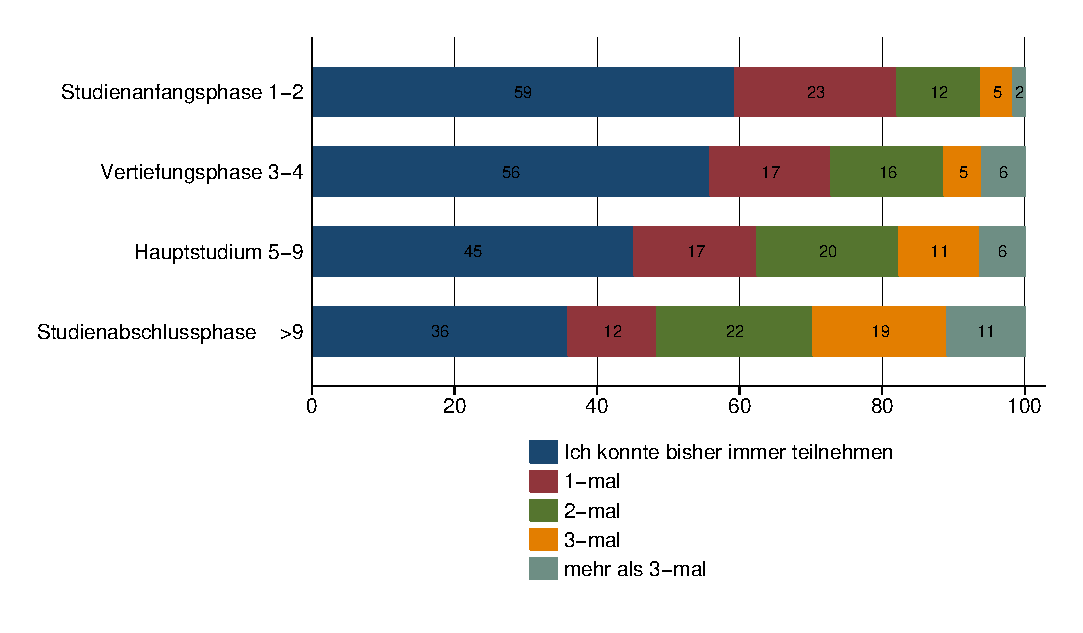
\includegraphics[width=.75\linewidth]{image}
%
% Some text added by hand.
% \caption{A \env{marginfigure}}
% \label{fig:marginfigure}
% \end{marginfigure}
% \end{dtxexample}
%
%
% \begin{dtxexample}[\Cref{fig:margintable}]{The \env{margintable} environment\label{ex:margintable}}
% \begin{margintable}
% \centering
% \testwidetable
% \caption{A \env{margintable}}
% \label{fig:margintable}
% \end{margintable}
% \end{dtxexample}
%
%
% \begin{dtxexample}[\Cref{fig:keyfigm}]{Using \cs{keyfig}\texttt{[M]}\label{ex:keyfigm}}
% \keyfig[M]{c={A \cs{keyfig}\texttt{[M]}},l=fig:keyfigm,ft,
% 	t=Additional text.
% 	Text text text text text text.
% 
% 	More paragraphs.
% }{image2}
% \end{dtxexample}
%
%
% \begin{dtxexample}[\Cref{tab:keytablem}]
%	{Using \env{keytable}\texttt{[M]} and an offset\label{ex:keytablem}}
% \begin{keytable}[M]{c={A \env{keytable}\texttt{[M]}},
% 	l=tab:keytablem,mo=-.9in}
% \testwidetable
% \end{keytable}
% \end{dtxexample}
%
% A negative offset was used to shift the table upwards
% \margintag{margin float offset}
% to the top of the example.
%
% To set the minimum-allowed distance between \cs{marginpar}s and margin floats:
% \margintag{distance between floats}
% \index{distance between floats}\index{float>distance between}
% \begin{verbatim}
% \setlength{\marginparpush}{3ex}
% \end{verbatim}
%
%
%
% \clearpage
% \subsubsection{Wrapped Floats}
% \changes{v0.12}{2016/12/03}{Docs: Wrapped float examples.}
%
% \begin{dtxexample}[\Cref{fig:keyfigw,tab:keytabw}]
%	{Using \cs{keyfig}\texttt{[W]} and \cs{keytab}\texttt{[W]}\label{ex:keyfigw}}
% \keyfig[W]{c={A \cs{keyfig}\texttt{[W]}},
% 	l=fig:keyfigw,ft,lw=.4,wp=I,
% 	t={.4\cs{linewidth} wide, placed \texttt{I}.}
% }{image2}
% \lipsum[1]
% \keytab[W]{c={A \cs{keytab}\texttt{[W]}},l=tab:keytabw,w=.75in,
% }{\testtable}
% \lipsum[2]
% \end{dtxexample}
%
% \begin{dtxexample}[\Cref{fig:keyfigboxw} and the \cs{keyparbox}.]
%	{Using \cs{keyfigbox}\texttt{[W]} and \cs{keyparbox}\texttt{[W]}\label{ex:keyfigboxw}}
% \keyfigbox[W]{c={A \cs{keyfigbox}\texttt{[W]}},
% 	l=fig:keyfigboxw,f,lw=.25,wp=I,
% 	t=Text text text text text text text text text
% }{The contents.}
% \lipsum[1]
% \keyparbox[W]{w=1in}{A \cs{keyparbox}[W] and some more text.}
% \lipsum[2]
% \end{dtxexample}
%
%
% \begin{dtxexample}[\Cref{fig:keyfigurew,tab:keytablew}]
%	{Using \cs{keyfigure}\texttt{[W]} and \cs{keytable}[W]\label{ex:keyfiguretablew}}
% \begin{keyfigure}[W]{c={A \cs{keyfigure}\texttt{[W]}},
% 	l=fig:keyfigurew,f,w=1.5in}
% This is a keyfigure.
% \end{keyfigure}
% \lipsum[1]
%
% \begin{keytable}[W]{c={A \env{keytable}\texttt{[W]}},
% 	l=tab:keytablew,w=2in,wp=L,tc=Placed \texttt{L} and 2in wide.}
% \testwidetable
% \end{keytable}
% \lipsum[2]
% \end{dtxexample}
%
%
% \clearpage
%
% \begin{dtxexample}[\Cref{fig:keywrapfig}]
%	{Using \cs{keywrap} with a \cs{keyfig}\label{ex:keywrapkeyfig}}
% \begin{itemize}
% \item First item.
%     Several lines of text text text text text
%     text text text text text text text text.
% \item \begin{keywrap}{.3\linewidth}{\keyfig{%
%       lw=1,c={Keywrap with \cs{keyfig}},l=fig:keywrapfig%
%     }{image}}
%         Second item.
%         Several lines of text text text text text
%         text text text text text text text text text
%         text text text text text text text.
%
%         These paragraphs are inside the \texttt{keywrap}.
%         A vertical gap appears below if the text is not enough to
%         fill the space next to the \cs{keyfig}.
%     \end{keywrap}
%     Outside the \env{wrapfig},\margintag{notes}\
%     but still in the second item.
%     There is no elegant way to place only part of a paragraph
%     inside a \env{keywrap}, and attempting to do so requires
%     manually removing the vertical paragraph skip.
% \item Third item.
% \end{itemize}
% \end{dtxexample}
%
%
%
% \clearpage
% \subsubsection{Custom Frames}
%
% 
% \begin{dtxexample}[\Cref{fig:customframe,fig:customlooseframe}]
%	{Custom frames with \pkg{mdframed}\label{ex:customframe}}
% \renewcommand{\KFLTtightframe}[1]{%
% \begin{minipage}{\KFLTimageboxwidth}
% \begin{mdtightframe}%
% #1
% \end{mdtightframe}%
% \end{minipage}
% }
% \setlength{\KFLTtightframewidth}{1pt}
%
% \renewcommand{\KFLTlooseframe}[1]{%
% \begin{mdlooseframe}[leftmargin=1.5in,rightmargin=1.5in]%
% #1
% \end{mdlooseframe}%
% }
% \setlength{\KFLTlooseframewidth}{4pt}
%
% \keyfig{ft,c=Custom-framed image,l=fig:customframe,r=90}{image}
% \keyfigbox{f,c=Custom loosely-framed box,
% 	l=fig:customlooseframe}{A loosely-framed box.}
% \end{dtxexample}
%
% \DescribePackage{mdframed}
% \Cref{ex:customframe} shows custom frames
% created with the \pkg{mdframed} package along with \pkg{tikz}.
% Note that \pkg{mdframed} uses the full \cs{linewidth}
% \watchout[\pkg{mdframed} width]
% even if the left/right margins are explicitly set, which
% causes extra vertical space when rotated.
% Because of this, the framed object is enclosed inside a minipage
% whose width is precomputed based on the object itself, then
% set in \cs{KFLTimageboxwidth}.  Any shadow may fall outside this
% box.
% \index{troubleshooting>rotating>extra space}
% \index{troubleshooting>mdframed}
%
% See \cref{sec:customframes} for more details.
%
% \begin{dtxexample}[\Cref{fig:customshadow,fig:customlooseshadow}]
%	{Custom shadows with \pkg{fancybox}\label{ex:customshadow}}
% \renewcommand{\KFLTtightframe}[1]{%
% \setlength{\fboxrule}{.4pt}
% \setlength{\fboxsep}{0pt}
% \setlength{\shadowsize}{2pt}
% \shadowbox{#1}%
% }
% \setlength{\KFLTtightframewidth}{0.4pt}
%
% \renewcommand{\KFLTlooseframe}[1]{%
% \setlength{\fboxrule}{.4pt}
% \setlength{\fboxsep}{3pt}
% \setlength{\shadowsize}{2pt}
% \shadowbox{#1}%
% }
% \setlength{\KFLTlooseframewidth}{3.4pt}
%
% \keyfig{ft,c=Custom shadow,l=fig:customshadow}{image}
% \keyfigbox{f,c=Custom loosely-framed shadow,lw=.5,
% 	l=fig:customlooseshadow}{A loosely-framed shadow box.}
% \end{dtxexample}
%
% \DescribePackage{fancybox}
% \Cref{ex:customshadow} shows custom shadow frames
% created with the \pkg{fancybox} package.
% This combination respects |lw| and |w|.
%
% See \cref{sec:customframes} for more details.
%
%
%
%
%
% \renewcommand{\KFLTtightframe}[1]{%
% \setlength{\fboxsep}{0pt}%
% \setlength{\fboxrule}{.4pt}%
% \fbox{#1}%
% }
% \setlength{\KFLTtightframewidth}{.4pt}
% 
% \renewcommand{\KFLTlooseframe}[1]{%
% \setlength{\fboxsep}{3pt}%
% \setlength{\fboxrule}{.4pt}%
% \fbox{#1}%
% }
% \setlength{\KFLTlooseframewidth}{3.4pt}
%
%
%
%
%
% \clearpage
% \subsubsection{Artist's Name}
%
% \begin{dtxexample}[\Cref{fig:artist}]{Artist's name — image}
% \keyfig{ft,ap=Mr.,af=First,al=Last,as={~III},
%	tc={\textit{About the illustration.}},
%	c=Artist's name — image,l=fig:artist}{image}
% \end{dtxexample}
%
%
% \begin{dtxexample}[\Cref{fig:artistpar}]{Artist's name — arbitrary contents}
% \tdnameright
% \begin{keyfigure}{f,ap=Mr.,al=Last,
%	c=Artist's name — arbitrary contents,l=fig:artistpar}
% \centering Some text, a quotation, a TikZ\ diagram —
% anything not an image file.
% \end{keyfigure}
% \tdnamecenter
% \end{dtxexample}
%
% The artist's name and optional prefix/suffix are printed below the figure,
% and an index entry is made for the name in (Last, First) format,
% or (Last) if there is no first name.
% If the \pkg{tocdata} package is loaded, the artist's name is also added to
% the List of Figures, and the \pkg{tocdata} \cs{tdname}\dots\ macros
% may be used to align the name.
%
%
%
% \begin{dtxexample}[\Cref{fig:artistcollection}]{Subfloats with an artist}
% \begin{keysubfigs}{2}{
% 	c=Artist's collection, l=fig:artistcollection,
% 	t={Some fully-justified text just for illustrative purposes,
% 	in case you have use for long explanations.
% 	This text may be the full \cs{linewidth} in size. \par
% 	Multiple paragraphs of text are allowed.},
% 	ap=Prefix,af=First,al=Last,as={, Suffix}
% }
% 	\keyfig{c=Artist's First Work}{image}
% 	\keyfig{c=Artist's Second Work,
% 		tc={Commentary about the work.}}{image2}
% \end{keysubfigs}
% \end{dtxexample}
%
% A group of figures may be placed into a subfloat container,
% which may have its own artist keys and additional text.
% Furthermore, each subfloat inside the collection may also have its
% own artist tags and additional text.
%
%
% \clearpage
%
% \subsection{Customization}
%
% \subsubsection{Custom Frames}
% \label{sec:customframes}
%
% \index{frame>custom}
%
% There are two user-redefinable framing macros: \\
% \hspace*{2em}\cs{KFLTtightframe} and \cs{KFLTlooseframe}
%
% A float's contents are placed into a box,
% which is passed to either of these two macros
% depending on the key |f| or |tf|.
%
% Each macro takes one argument and frames it.
%
% Each macro has an associated \LaTeX\ length: \\
% \hspace*{2em}\cs{KFLTtightframewidth} and \cs{KFLTlooseframewidth}
%
% These lengths must be redefined to the expected
% total frame width, equal to the frame thickness plus
% separation.
%
% The defaults definitions are:
% \begin{Verbatim}[gobble=2]
% \newcommand{\KFLTtightframe}[1]{%
% \setlength{\fboxsep}{0pt}%
% \setlength{\fboxrule}{.4pt}%
% \fbox{#1}%
% }
% \setlength{\KFLTtightframewidth}{.4pt}
% 
% \newcommand{\KFLTlooseframe}[1]{%
% \setlength{\fboxsep}{3pt}%
% \setlength{\fboxrule}{.4pt}%
% \fbox{#1}%
% }
% \setlength{\KFLTlooseframewidth}{3.4pt}
% \end{Verbatim}
%
% See \cref{ex:customframe} for an example
% created with the \pkg{mdframed} package,
% and \cref{ex:customshadow} for an example
% created with the \pkg{fancybox} package.
%
%
%
% \subsubsection{Distance between Floats and Rows}
% \index{distance between floats}
% \index{subfloat>distance between}
% \index{float>distance between}
% \index{troubleshooting>rows too close or far}
% To spread out the distance between floats and/or rows of floats
% \margintag{rows too close/far}
% on a busy page, the following adjustments may be made.
% The values used in this documentation are:
% \begin{verbatim}
% \setlength{\floatsep}{5ex plus 1ex minus 1ex}
% \setlength{\dblfloatsep}{5ex plus 1ex minus 1ex}
% \end{verbatim}
%
%
% \subsubsection{Formatting the Captions}
%
% \index{troubleshooting>caption format}
% To modify the typesetting of the captions, see the \pkg{caption} package.
% \index{caption>formatting}
% The settings used in this documentation are:
% \begin{verbatim}
% % default applied to margin floats:
% \captionsetup{labelfont={small,bf},textfont={small,bf}}
% 
% \captionsetup[figure]{
% 	style=default, justification=centering,
% 	margin=0pt, parskip=0pt, skip=2ex,
% 	labelfont={small,bf},textfont={small,bf}
% }
% 
% \captionsetup[table]{
% 	style=default, justification=centering,
% 	margin=0pt, parskip=0pt, skip=1ex,
% 	labelfont={small,bf},textfont={small,bf}
% }
% 
% \captionsetup[subfigure]{
% 	style=default, justification=centering,
% 	margin=0pt, parskip=0pt, skip=2ex,
% 	labelfont={small},textfont={small}
% }
% 
% \captionsetup[subtable]{
% 	style=default, justification=centering,
% 	margin=0pt, parskip=0pt, skip=1ex,
% 	labelfont={small},textfont={small}
% }
% \end{verbatim}



% \clearpage
%
% \StopEventually{\PrintChanges\PrintIndex}
% 
%
%
% \section{Code}
%
%
%
%
%
%
% \subsection{Required Packages}
%
% \DescribePackage{etoolbox} v2.6 or later
%	for \cs{BeforeBeginEnvironment}, \cs{AfterEndEnvironment}
%    \begin{macrocode}
\RequirePackage{etoolbox}[2011/01/03]%

\RequirePackage{xparse}

\RequirePackage{xifthen}
%    \end{macrocode}
% \DescribePackage{keyval} Key processing:
%    \begin{macrocode}
\RequirePackage{xkeyval}
%    \end{macrocode}
% \DescribePackage{graphicx} For \cs{includegraphics} and \pkg{rotating}:
%    \begin{macrocode}
\RequirePackage{graphicx}
%    \end{macrocode}
% \DescribePackage{caption} Handles all caption-related functions:
%    \begin{macrocode}
\RequirePackage{caption}[2010/10/31]% v3.2 to support \phantomcaption
%    \end{macrocode}
% \DescribePackage{subcaption} Derived from \pkg{caption}, used to handle subfloats:
%    \begin{macrocode}
\RequirePackage{subcaption}
%    \end{macrocode}
% \DescribePackage{calc} Used to compute box width minus frame sep and width.
%    \begin{macrocode}
\RequirePackage{calc}
%    \end{macrocode}
% \DescribePackage{rotating} Provides rotation via the \env{turn} environment:
%    \begin{macrocode}
\RequirePackage{rotating}
%    \end{macrocode}
% \DescribePackage{placeins} Provides \FloatBarrier to process existing floats before adding new ones.
%    \begin{macrocode}
\RequirePackage{placeins}
%    \end{macrocode}
% \DescribePackage{wrapfig} Provides figure wrapping code.
%    \begin{macrocode}
\RequirePackage{wrapfig}
%    \end{macrocode}
%
%
% Package error if floatrow was loaded:
%
% \changes{v0.13}{2017/01/12}{Error if \pkg{floatrow} was loaded.}
%
%    \begin{macrocode}
\@ifpackageloaded{floatrow}
{
\PackageError{keyfloat}
{The keyfloat conflicts with the floatrow package.
Remove floatrow to use keyfloat.}
{Keyfloat uses the caption and subcaption packages to
provide similar functionality to floatrow.}
}
{}
%    \end{macrocode}



%
% \DescribePackage{gettitlestring} Used by \pkg{hyperref} and \pkg{nameref}.
%
% \changes{v0.13}{2017/01/14}{Fix: Expands names in references.}
%
% Expand names used in titles:
%    \begin{macrocode}
\PassOptionsToPackage{expand}{gettitlestring}
%    \end{macrocode}


% Rows of floats are created by a simple \env{minipage} environment,
% instead of relying on a preexisting package.  This proved to be
% advantageous when support was added for multiple rows in one
% environment.
%

% \subsection{In-line Figures and Tables}

% These macros are commonly used by others.

% \begin{environment}{tablehere} Place a table exactly [H].
%    \begin{macrocode}
\ProvideDocumentEnvironment{tablehere}{}
  {\bigbreak\noindent\minipage{\linewidth}\def\@captype{table}}
  {\endminipage\bigbreak}
%    \end{macrocode}
% \end{environment}

% \begin{environment}{figurehere} Place a figure exactly [H].
%    \begin{macrocode}
\ProvideDocumentEnvironment{figurehere}{}
  {\bigbreak\noindent\minipage{\linewidth}\def\@captype{figure}}
  {\endminipage\bigbreak}
%    \end{macrocode}
% \end{environment}



% \subsection{Row Counting and Control}

% Used to count position and wrap at end of each row.


% \DescribeCounter{KFLT@numcols} Columns per row.
%    \begin{macrocode}
\newcounter{KFLT@numcols}
%    \end{macrocode}

% \DescribeCounter{KFLT@thiscol} Column currently processing.
% |0| if not yet in a keyfloats or subfloat.
%
%    \begin{macrocode}
\newcounter{KFLT@thiscol}
%    \end{macrocode}

% \DescribeLength{\KFLT@rowboxwidth} How wide is each box in the row.
%    \begin{macrocode}
\newlength{\KFLT@rowboxwidth}
%    \end{macrocode}





% \subsection{Float Key Handling}

% \DescribeBoolean{KFLT@cont} Continued float?
%    \begin{macrocode}
\newboolean{KFLT@cont}
%    \end{macrocode}
%
% \DescribeKey[main]{cont} Continued float?
%
%    \begin{macrocode}
\define@key{KFLT@keys}{cont}[true]{\setboolean{KFLT@cont}{#1}}
%    \end{macrocode}
%
% \begin{macro}{\KFLT@c} Caption storage
%    \begin{macrocode}
\newcommand{\KFLT@c}{}
%    \end{macrocode}
% \end{macro}
%
% \DescribeBoolean{KFLT@cstar} Starred caption?
%    \begin{macrocode}
\newboolean{KFLT@cstar}
%    \end{macrocode}
%
% \DescribeKey[main]{c} Caption
%
%    \begin{macrocode}
\define@key{KFLT@keys}{c}%
	{\renewcommand{\KFLT@c}{#1}\setboolean{KFLT@cstar}{false}}
%    \end{macrocode}
%
% \DescribeKey[main]{cstar} Caption starred?
%
%    \begin{macrocode}
\define@key{KFLT@keys}{cstar}%
	{\renewcommand{\KFLT@c}{#1}\setboolean{KFLT@cstar}{true}}
%    \end{macrocode}
%
% \DescribeKey[main]{sc} Short caption
%
%    \begin{macrocode}
\define@key{KFLT@keys}{sc}{%
\renewcommand{\KFLT@sc}{#1}%
\setboolean{KFLT@scgiven}{true}%
}
%    \end{macrocode}
%
% \begin{macro}{\KFLT@sc} Short caption storage
%    \begin{macrocode}
\newcommand{\KFLT@sc}{}
%    \end{macrocode}
% \end{macro}
%
% \DescribeBoolean{KFLT@scgiven} Was a short caption given?
%    \begin{macrocode}
\newboolean{KFLT@scgiven}
%    \end{macrocode}
%
% \begin{macro}{\KFLT@type} Float type: ``|figure|'', ``|table|''
%    \begin{macrocode}
\newcommand*{\KFLT@type}{}
%    \end{macrocode}
% \end{macro}
%
% \begin{macro}{\KFLT@listtype} List type: ``|lof|'', ``|lot|''
%    \begin{macrocode}
\newcommand*{\KFLT@listtype}{}
%    \end{macrocode}
% \end{macro}
%
%
% \DescribeKey[main]{l} Label
%    \begin{macrocode}
\define@key{KFLT@keys}{l}{\renewcommand{\KFLT@l}{#1}}
%    \end{macrocode}
%
% \begin{macro}{\KFLT@l} Label storage
%    \begin{macrocode}
\newcommand*{\KFLT@l}{}
%    \end{macrocode}
% \end{macro}
%
%
% For the artist/author keys:
%
% \DescribeKey[main]{ap} Artist prefix
%    \begin{macrocode}
\define@key{KFLT@keys}{ap}{\renewcommand{\KFLT@ap}{#1}}
%    \end{macrocode}
%
% \begin{macro}{\KFLT@ap} Storage for artist prefix
%    \begin{macrocode}
\newcommand*{\KFLT@ap}{}
%    \end{macrocode}
% \end{macro}
%
% \DescribeKey[main]{af} Artist first name
%    \begin{macrocode}
\define@key{KFLT@keys}{af}{\renewcommand{\KFLT@af}{#1}}
%    \end{macrocode}
%
% \begin{macro}{\KFLT@af} Storage for artist first name
%    \begin{macrocode}
\newcommand*{\KFLT@af}{}
%    \end{macrocode}
% \end{macro}
%
% \DescribeKey[main]{al} Artist last name
%    \begin{macrocode}
\define@key{KFLT@keys}{al}{\renewcommand{\KFLT@al}{#1}}
%    \end{macrocode}
%
% \begin{macro}{\KFLT@al} Storage for artist last name
%    \begin{macrocode}
\newcommand*{\KFLT@al}{}
%    \end{macrocode}
% \end{macro}
%
% \DescribeKey[main]{as} Artist suffix
%    \begin{macrocode}
\define@key{KFLT@keys}{as}{\renewcommand{\KFLT@as}{#1}}
%    \end{macrocode}
%
% \begin{macro}{\KFLT@as} Storage for artist suffix
%    \begin{macrocode}
\newcommand*{\KFLT@as}{}
%    \end{macrocode}
% \end{macro}
%
%
%
%
%
%
% \begin{macro}{\KFLT@textalign} Storage for text alignment.
%
% Used for the additional text in the float.
%    \begin{macrocode}
\newcommand*{\KFLT@textalign}{}
%    \end{macrocode}
% \end{macro}
%
% \begin{macro}{\KFLT@t} Additional text storage
%
% Used for the additional text in the float.
%    \begin{macrocode}
\newcommand{\KFLT@t}{}
%    \end{macrocode}
% \end{macro}
%
%
% Create replacement macros in case \pkg{tocdata} is not loaded:
% \changes{v0.12}{2016/12/02}{Adapts to older version of tocdata.}
%    \begin{macrocode}
\providecommand{\tdtextjustify}{}
\providecommand{\tdtextcenter}{}
\providecommand{\tdtextleft}{}
\providecommand{\tdtextright}{}
\providecommand{\tdnamejustify}{}
\providecommand{\tdnamecenter}{}
\providecommand{\tdnameleft}{}
\providecommand{\tdnameright}{}
%    \end{macrocode}
%
% \DescribeKey[main]{t} Additional text, justified alignment.
%    \begin{macrocode}
\define@key{KFLT@keys}{t}{
\renewcommand{\KFLT@t}{#1}
\renewcommand{\KFLT@textalign}{}
\tdtextjustify
}
%    \end{macrocode}
%
% \DescribeKey[main]{tc} Additional text, centered alignment.
%    \begin{macrocode}
\define@key{KFLT@keys}{tc}{
\renewcommand{\KFLT@t}{#1}
\renewcommand{\KFLT@textalign}{\centering}
\tdtextcenter
}
%    \end{macrocode}
%
% \DescribeKey[main]{tr} Additional text, aligned to the right.
%    \begin{macrocode}
\define@key{KFLT@keys}{tr}{
\renewcommand{\KFLT@t}{#1}
\renewcommand{\KFLT@textalign}{\raggedleft}
\tdtextright
}
%    \end{macrocode}
%
% \DescribeKey[main]{tl} Additional text, aligned to the left.
%    \begin{macrocode}
\define@key{KFLT@keys}{tl}{
\renewcommand{\KFLT@t}{#1}
\renewcommand{\KFLT@textalign}{\raggedright}
\tdtextleft
}
%    \end{macrocode}
%
%
%
% \begin{macro}{\KFLT@i} Image filename storage
%    \begin{macrocode}
\newcommand*{\KFLT@i}{}
%    \end{macrocode}
% \end{macro}
%
%
% \DescribeKey[main]{lw} Fraction of \cs{linewidth}
%    \begin{macrocode}
\define@key{KFLT@keys}{lw}{%
\renewcommand{\KFLT@lw}{#1}%
\setlength{\KFLT@w}{0pt}%
}
%    \end{macrocode}
%
% \begin{macro}{\KFLT@lw} Fraction of linewidth storage: ``|.5|''
%    \begin{macrocode}
\newcommand*{\KFLT@lw}{}
%    \end{macrocode}
% \end{macro}
%
% \DescribeKey[main]{w} Fixed width
%    \begin{macrocode}
\define@key{KFLT@keys}{w}{%
\setlength{\KFLT@w}{#1}%
\renewcommand{\KFLT@lw}{}%
}
%    \end{macrocode}
%
% \begin{macro}{\KFLT@w} Width storage: ``3cm''
%    \begin{macrocode}
\newlength{\KFLT@w}
%    \end{macrocode}
% \end{macro}
%
% \DescribeKey[main]{h} Fixed height
%    \begin{macrocode}
\define@key{KFLT@keys}{h}{\setlength{\KFLT@h}{#1}}
%    \end{macrocode}
%
% \begin{macro}{\KFLT@h} Height storage: ``2in''
%    \begin{macrocode}
\newlength{\KFLT@h}
%    \end{macrocode}
% \end{macro}
%
% \DescribeKey[main]{s} Scale
%    \begin{macrocode}
\define@key{KFLT@keys}{s}{\renewcommand{\KFLT@s}{#1}}
%    \end{macrocode}
%
% \begin{macro}{\KFLT@s} Scale storage: ``3''
%    \begin{macrocode}
\newcommand*{\KFLT@s}{1}
%    \end{macrocode}
% \end{macro}
%
% \DescribeKey[main]{r} Angle.  90 is counter-clockwise 90 degrees.
%    \begin{macrocode}
\define@key{KFLT@keys}{r}{\renewcommand{\KFLT@r}{#1}}
%    \end{macrocode}
%
% \begin{macro}{\KFLT@r} Angle storage: ``90''
%    \begin{macrocode}
\newcommand*{\KFLT@r}{0}
%    \end{macrocode}
% \end{macro}
%
% \DescribeKey[main]{f} Frame the image with \cs{KFLTlooseframe}.
%    \begin{macrocode}
\define@key{KFLT@keys}{f}[true]{\setboolean{KFLT@f}{#1}}
%    \end{macrocode}
%
% \DescribeBoolean{KFLT@f} Frame the image?
%    \begin{macrocode}
\newboolean{KFLT@f}
%    \end{macrocode}

% \DescribeKey[main]{ft} Tightly frame the image using \cs{KFLTtightframe}.
%	This is useful for photographs, or diagrams which
%	already have built-in margins.
%    \begin{macrocode}
\define@key{KFLT@keys}{ft}[true]{\setboolean{KFLT@ft}{#1}}
%    \end{macrocode}
%
% \DescribeBoolean{KFLT@ft} Tightly frame the image?
%    \begin{macrocode}
\newboolean{KFLT@ft}
%    \end{macrocode}


% \DescribeKey[main]{stretch} Set \cs{arraystretch} inside the table environment.
%    \begin{macrocode}
\define@key{KFLT@keys}{stretch}{\renewcommand{\KFLT@stretch}{#1}}
%    \end{macrocode}
%
% \begin{macro}{\KFLT@stretch} Storage for \cs{arraystretch}.
%    \begin{macrocode}
\newcommand*{\KFLT@stretch}{1}
%    \end{macrocode}
% \end{macro}


% \DescribeKey[main]{mo} Set vertical offset for a margin float.
% \changes{v0.12}{2016/12/03}{Added \texttt{mo} key.}
%    \begin{macrocode}
\define@key{KFLT@keys}{mo}{\setlength{\KFLT@mo}{#1}}
%    \end{macrocode}
%
% \begin{macro}{\KFLT@mo} Storage for the vertical margin offset.
%    \begin{macrocode}
\newlength{\KFLT@mo}
%    \end{macrocode}
% \end{macro}


% \DescribeKey[main]{wp} Set wrap placement for a wrapped float.
%
% See \cref{tab:wrapplacement} on \cpageref{tab:wrapplacement}.
% 
% \changes{v0.12}{2016/12/03}{Added \texttt{wp} key.}
%    \begin{macrocode}
\define@key{KFLT@keys}{wp}{\renewcommand{\KFLT@wp}{#1}}
%    \end{macrocode}
%
% \begin{macro}{\KFLT@wp} Storage for the wrap placement.
%    \begin{macrocode}
\newcommand{\KFLT@wp}{O}
%    \end{macrocode}
% \end{macro}


% \DescribeKey[main]{va} Set vertical alignment of the outermost minipage container.
%
% \changes{v0.15}{2017/05/09}{Added vertical alignment key \texttt{va}.}
%    \begin{macrocode}
\define@key{KFLT@keys}{va}{\renewcommand{\KFLT@va}{#1}}
%    \end{macrocode}
%
% \begin{macro}{\KFLT@va} Storage for the vertical alignment.
%    \begin{macrocode}
\newcommand{\KFLT@va}{c}
%    \end{macrocode}
% \end{macro}





% \subsection{Nesting Control}

% \DescribeCounter{KFLT@keyfloatdepth} Depth inside a keyfigs environment
%    \begin{macrocode}
\newcounter{KFLT@keyfloatdepth}
\setcounter{KFLT@keyfloatdepth}{0}
%    \end{macrocode}

% \DescribeBoolean{KFLT@inkeysubfloats} Inside a keysubfigs environment?
%    \begin{macrocode}
\newboolean{KFLT@inkeysubfloats}
\setboolean{KFLT@inkeysubfloats}{false}
%    \end{macrocode}



% \subsection{Subfloat Key Handling}
%
% These keys are for the container holding a collection of subfigures.

% \DescribeBoolean{KFLT@subgrpcont} Continued float?
%    \begin{macrocode}
\newboolean{KFLT@subgrpcont}{}
%    \end{macrocode}
%
% \DescribeKey[subfloat container]{cont} Continued float
%    \begin{macrocode}
\define@key{KFLT@subgrpkeys}{cont}[true]{%
\setboolean{KFLT@subgrpcont}{#1}%
}
%    \end{macrocode}

% \begin{macro}{\KFLT@subgrpc} Sub-caption storage
%    \begin{macrocode}
\newcommand{\KFLT@subgrpc}{}
%    \end{macrocode}
% \end{macro}

% \DescribeBoolean{KFLT@subgrpcstart} Sub-caption starred?
%    \begin{macrocode}
\newboolean{KFLT@subgrpcstar}
%    \end{macrocode}
%
% \DescribeKey[subfloat container]{c} Caption
%    \begin{macrocode}
\define@key{KFLT@subgrpkeys}{c}
	{\renewcommand{\KFLT@subgrpc}{#1}\setboolean{KFLT@subgrpcstar}{false}}
%    \end{macrocode}
%
% \DescribeKey[subfloat container]{cstar} Starred caption?
%    \begin{macrocode}
\define@key{KFLT@subgrpkeys}{cstar}
	{\renewcommand{\KFLT@subgrpc}{#1}\setboolean{KFLT@subgrpcstar}{true}}
%    \end{macrocode}
%
% \DescribeKey[subfloat container]{sc} Short caption
%    \begin{macrocode}
\define@key{KFLT@subgrpkeys}{sc}{%
\renewcommand{\KFLT@subgrpsc}{#1}%
\setboolean{KFLT@subgrpscgiven}{true}%
}
%    \end{macrocode}

% \begin{macro}{\KFLT@subgrpsc} Sub-shortcaption storage
%    \begin{macrocode}
\newcommand{\KFLT@subgrpsc}{}
%    \end{macrocode}
% \end{macro}

% \DescribeBoolean{KFLT@subgrpscgiven} Sub-shortcaption was given?
%    \begin{macrocode}
\newboolean{KFLT@subgrpscgiven}
%    \end{macrocode}

% \begin{macro}{\KFLT@subgrptype} Subfloats collection type storage:
%	``|figure|'', ``|table|''
%    \begin{macrocode}
\newcommand*{\KFLT@subgrptype}{}
%    \end{macrocode}
% \end{macro}

% \begin{macro}{\KFLT@subgrptype} Subfloats collection list type storage:
%	``|lof|'', ``|lot|''
%    \begin{macrocode}
\newcommand*{\KFLT@subgrplisttype}{}
%    \end{macrocode}
% \end{macro}

% \begin{macro}{\KFLT@setsubgrpfigure} Set to figure type
%    \begin{macrocode}
\newcommand*{\KFLT@setsubgrpfigure}{%
\renewcommand{\KFLT@subgrptype}{figure}%
\renewcommand{\KFLT@subgrplisttype}{lof}%
}
%    \end{macrocode}
% \end{macro}

% \begin{macro}{\KFLT@setsubgrptable} Set to table type
%    \begin{macrocode}
\newcommand*{\KFLT@setsubgrptable}{%
\renewcommand{\KFLT@subgrptype}{table}%
\renewcommand{\KFLT@subgrplisttype}{lot}%
}
%    \end{macrocode}
% \end{macro}
%
%
% \DescribeKey[subfloat container]{l} Label
%    \begin{macrocode}
\define@key{KFLT@subgrpkeys}{l}{\renewcommand{\KFLT@subgrpl}{#1}}
\newcommand*{\KFLT@subgrpl}{}
%    \end{macrocode}
%
%
%
% \begin{macro}{\KFLT@subgrptextalign} Storage for text alignment.
%
% Used for the additional text in the float.
%    \begin{macrocode}
\newcommand*{\KFLT@subgrptextalign}{}
%    \end{macrocode}
% \end{macro}
%
% \begin{macro}{\KFLT@subgrpt} Additional text storage
%
% Used for the additional text in the float.
%    \begin{macrocode}
\newcommand{\KFLT@subgrpt}{}
%    \end{macrocode}
% \end{macro}
%
%
% \DescribeKey[subfloat container]{t} Additional text — full justification
%    \begin{macrocode}
\define@key{KFLT@subgrpkeys}{t}{
\renewcommand{\KFLT@subgrpt}{#1}
\renewcommand{\KFLT@subgrptextalign}{}
\tdtextjustify
}
%    \end{macrocode}
%
% \DescribeKey[subfloat container]{t} Additional text — center justification
%    \begin{macrocode}
\define@key{KFLT@subgrpkeys}{tc}{
\renewcommand{\KFLT@subgrpt}{#1}
\renewcommand{\KFLT@subgrptextalign}{\centering}
\tdtextcenter
}
%    \end{macrocode}
%
% \DescribeKey[subfloat container]{t} Additional text — aligned left
%    \begin{macrocode}
\define@key{KFLT@subgrpkeys}{tl}{
\renewcommand{\KFLT@subgrpt}{#1}
\renewcommand{\KFLT@subgrptextalign}{\raggedright}
\tdtextleft
}
%    \end{macrocode}
%
% \DescribeKey[subfloat container]{t} Additional text — aligned right
%    \begin{macrocode}
\define@key{KFLT@subgrpkeys}{tr}{
\renewcommand{\KFLT@subgrpt}{#1}
\renewcommand{\KFLT@subgrptextalign}{\raggedleft}
\tdtextright
}
%    \end{macrocode}
%
%
%
% For the \pkg{tocdata} package:
%
% \DescribeKey[subfloat container]{ap} Artist prefix
%    \begin{macrocode}
\define@key{KFLT@subgrpkeys}{ap}{\renewcommand{\KFLT@subgrpap}{#1}}
%    \end{macrocode}
%
% \begin{macro}{\KFLT@subgrpap} Storage for artist prefix
%    \begin{macrocode}
\newcommand*{\KFLT@subgrpap}{}
%    \end{macrocode}
% \end{macro}
%
% \DescribeKey[subfloat container]{af} Artist first name
%    \begin{macrocode}
\define@key{KFLT@subgrpkeys}{af}{\renewcommand{\KFLT@subgrpaf}{#1}}
%    \end{macrocode}
%
% \begin{macro}{\KFLT@subgrpaf} Storage for artist first name
%    \begin{macrocode}
\newcommand*{\KFLT@subgrpaf}{}
%    \end{macrocode}
% \end{macro}
%
% \DescribeKey[subfloat container]{al} Artist last name
%    \begin{macrocode}
\define@key{KFLT@subgrpkeys}{al}{\renewcommand{\KFLT@subgrpal}{#1}}
%    \end{macrocode}
%
% \begin{macro}{\KFLT@subgrpal} Storage for artist last name
%    \begin{macrocode}
\newcommand*{\KFLT@subgrpal}{}
%    \end{macrocode}
% \end{macro}
%
% \DescribeKey[subfloat container]{as} Artist suffix
%    \begin{macrocode}
\define@key{KFLT@subgrpkeys}{as}{\renewcommand{\KFLT@subgrpas}{#1}}
%    \end{macrocode}
%
% \begin{macro}{\KFLT@subgrpas} Storage for artist suffix
%    \begin{macrocode}
\newcommand*{\KFLT@subgrpas}{}
%    \end{macrocode}
% \end{macro}
%%
%
%
%
%
%
%
%
%


% \subsection{Computing Image Width}

% \DescribeLength{\KFLT@imagewidth} Computed width of the image
%    \begin{macrocode}
\newlength{\KFLT@imagewidth}
%    \end{macrocode}

% \DescribeLength{\KFLT@boxwidth} Computed width of the container box
%    \begin{macrocode}
\newlength{\KFLT@boxwidth}
%    \end{macrocode}
%
%
%
%
%
% \begin{macro}{\KFLT@findwidths} Figure out how wide to make an image and its container
%    \begin{macrocode}
\newcommand*{\KFLT@findwidths}{%
%    \end{macrocode}
% Default to a box of full \cs{linewidth} minus the potential frame:
%    \begin{macrocode}
\ifthenelse{\boolean{KFLT@ft}}% tight frame?
{\setlength{\KFLT@boxwidth}{\linewidth - 2\KFLTtightframewidth}}%
{% not tight frame
\ifthenelse{\boolean{KFLT@f}}% loose frame?
{\setlength{\KFLT@boxwidth}{\linewidth - 2\KFLTlooseframewidth}}%
{\setlength{\KFLT@boxwidth}{\linewidth}}% no frame
}% not tight frame
%    \end{macrocode}
% Several width options exist.  First see if width was given:
%    \begin{macrocode}
\ifthenelse{\dimtest{\KFLT@w}{>}{0pt}}%
%    \end{macrocode}
%  Width was given:
%    \begin{macrocode}
{\setlength{\KFLT@imagewidth}{\KFLT@w}}%
{% width not given
%    \end{macrocode}
% Use full \cs{linewidth} or only a fraction:
%    \begin{macrocode}
\ifcsempty{\KFLT@lw}%
{\setlength{\KFLT@imagewidth}{\KFLT@boxwidth}}%
{\setlength{\KFLT@imagewidth}{\KFLT@lw\KFLT@boxwidth}}%
}% width not given
}
%    \end{macrocode}
% \end{macro}
%
%
% \subsection{Framing and Rotation}
%
%
% A user-redefinable macro and length to tightly frame the contents.
%
% \cs{KFLTtightframe} may be redefined to a macro which frames its contents.
% \cs{KFLTtightframewidth} should be redefine to the total width of the new
% frame and its separation.
%
% \begin{macro}{\KFLT@tightframe} \marg{contents}
%    \begin{macrocode}
\newcommand{\KFLTtightframe}[1]{%
\setlength{\fboxsep}{0pt}%
\setlength{\fboxrule}{.4pt}%
\fbox{#1}%
}

%    \end{macrocode}
% \end{macro}
%
% \DescribeLength{\KFLTtightframewidth} Combined width of the frame and separation.
%    \begin{macrocode}
\newlength{\KFLTtightframewidth}
\setlength{\KFLTtightframewidth}{.4pt}
%    \end{macrocode}
%
%
% \begin{macro}{\KFLTlooseframe} \marg{contents}
%
% A user-redefinable macro and length to loosely frame the contents.
%
% \cs{KFLTlooseframe} may be redefined to a macro which frames its contents.
% \cs{KFLTlooseframewidth} should be redefine to the total width of the new
% frame and its separation.
%
%    \begin{macrocode}
\newcommand{\KFLTlooseframe}[1]{%
\setlength{\fboxsep}{3pt}%
\setlength{\fboxrule}{.4pt}%
\fbox{#1}%
}
%    \end{macrocode}
% \end{macro}
%
% \DescribeLength{\KFLTlooseframewidth} Combined width of the frame and separation.
%    \begin{macrocode}
\newlength{\KFLTlooseframewidth}
\setlength{\KFLTlooseframewidth}{3.4pt}
%    \end{macrocode}
%
%
% \begin{macro}{\KFLT@frame} \marg{contents}
%
% Frames the contents according to the |f| key.  To be nested for further processing.
%    \begin{macrocode}
\newcommand{\KFLT@frame}[1]
{%
\ifthenelse{\boolean{KFLT@ft}}%
{\KFLTtightframe{#1}}%
{% not tightframe
\ifthenelse{\boolean{KFLT@f}}%
{\KFLTlooseframe{#1}}%
{#1}% no frame
}% not looseframe
}
%    \end{macrocode}
% \end{macro}
%
%
% \begin{macro}{KFLT@findenvboxwidth}
% Figures the width of the contents of \cs{KFLT@envbox} plus the frame:
%    \begin{macrocode}
\newcommand{\KFLT@findenvboxwidth}{%
\settowidth{\KFLTimageboxwidth}{\usebox{\KFLT@envbox}}%
\ifthenelse{\boolean{KFLT@ft}}%
{\addtolength{\KFLTimageboxwidth}{2\KFLTtightframewidth}}%
{% not tightframe
\ifthenelse{\boolean{KFLT@f}}%
{\addtolength{\KFLTimageboxwidth}{2\KFLTlooseframewidth}}%
{}% no frame
}% not looseframe
}
%    \end{macrocode}
% \end{macro}
%
%
%
%
% \subsection{A Graphics Image from a File}
%
% \begin{macro}{\KFLT@onefigureimage} Create a stand-alone figure with an image.
%    \begin{macrocode}
\NewDocumentCommand{\KFLT@onefigureimage}{}
{%
%    \end{macrocode}
% Several possible combinations of linewidth, width, and height are available,
% and each is treated separately.
% Scaling and width/height are done first, then framing, then rotation.
%    \begin{macrocode}
\begin{lrbox}{\KFLT@envbox}%
%    \end{macrocode}
% Handle the |lw| key.  If |lw| is used, width and height are ignored.
%    \begin{macrocode}
\ifthenelse{\NOT\equal{\KFLT@lw}{}}%
{\includegraphics%
[scale=\KFLT@s,width=\KFLT@imagewidth]{\KFLT@i}}%
{% not linewidth
%    \end{macrocode}
% Handle the |w| key, which may be used along with the |h| key:
%    \begin{macrocode}
\ifthenelse{\dimtest{\KFLT@w}{>}{0pt}}%
{% width is given
\ifthenelse{\dimtest{\KFLT@h}{>}{0pt}}%
%    \end{macrocode}
% Width and height are both given:
%    \begin{macrocode}
{% w and h
\includegraphics%
[scale=\KFLT@s,%
width=\KFLT@imagewidth,height=\KFLT@h]{\KFLT@i}%
}% w and h
%    \end{macrocode}
% Only width:
%    \begin{macrocode}
{% only w
\includegraphics%
[scale=\KFLT@s,width=\KFLT@imagewidth]{\KFLT@i}%
}% only w
}% width is given
%    \end{macrocode}
% Width was not given, so maybe handle |h| alone:
%    \begin{macrocode}
{% width is not given
\ifthenelse{\dimtest{\KFLT@h}{>}{0pt}}%
%    \end{macrocode}
% |h| was given:
%    \begin{macrocode}
{\includegraphics%
[scale=\KFLT@s,height=\KFLT@h]{\KFLT@i}}%
%    \end{macrocode}
% If none were given, use the image's natural size:
%    \begin{macrocode}
{\includegraphics%
[scale=\KFLT@s]{\KFLT@i}}%
}% width is not given
}% not linewidth
\end{lrbox}%
\unskip%
\KFLT@findenvboxwidth%
\begin{turn}{\KFLT@r}%
%    \end{macrocode}
% Encapsulate the frame in case the
% custom frame commands used pars:
%    \begin{macrocode}
% \begin{minipage}{\KFLTimageboxwidth}%
\KFLT@frame{\usebox{\KFLT@envbox}}%
% \end{minipage}%
\unskip%
\end{turn}%
}
%    \end{macrocode}
% \end{macro}




% \subsection{Printing the Caption}
%
%
% \begin{macro}{\KFLT@captioniftype} \marg{|figure| or |table|} \marg{\mainsubarg}
%
% Create a caption only if is of this float type.
%
% The second argument is |{}| if a regular float, or
% |subgrp| if \cs{keysubfigs} or \cs{keysubtabs}.
%    \begin{macrocode}
\newcommand*{\KFLT@captioniftype}[2]{%
\ifthenelse{\equal{\csname KFLT@#2type\endcsname}{#1}}%
{\KFLT@caption{#2}}%
{}%
}
%    \end{macrocode}
% \end{macro}




% \begin{macro}{\KFLT@dosimplecaption} \marg{star?} \marg{short cap or |-NO VALUE-|} \marg{caption}
%
% Calls \cs{caption} depending on several combinations of star and short captions
% being given.
%    \begin{macrocode}
\NewDocumentCommand{\KFLT@dosimplecaption}{m m m}
{%
\unskip%
\IfBooleanTF{#1}% star?
{% star
\IfValueTF{#2}{\caption*[#2]{#3}}{\caption*{#3}}%
}% star
{% no star
\IfValueTF{#2}{\caption[#2]{#3}}{\caption{#3}}%
}% no star
}
%    \end{macrocode}
% \end{macro}
%
%
%
% \begin{macro}{\KFLT@docaption} * \oarg{short caption} \marg{caption} \marg{\mainsubarg}
%
% Depending on whether the \pkg{tocdata} package is present,
% and an artist is specified,
% use either \cs{caption} or \cs{captionartist}.
%
% The fourth argument is |{}| if a regular float, or
% |subgrp| if \cs{keysubfigs} or \cs{keysubtabs}.
%
% See Table \ref{tab:captions} for the possible combinations of
% the caption-related keys: |c|, |cstar|, and |sc|.
%
% \changes{v0.14}{2017/02/09}{Fix: No index entry if no artist given.}
%
% There are two versions, depending on whether \pkg{tocdata} is loaded.
%    \begin{macrocode}
\@ifpackageloaded{tocdata}
{% tocdata loaded
%    \end{macrocode}
% \pkg{tocdata} is loaded:
%    \begin{macrocode}
\NewDocumentCommand{\KFLT@docaption}{s o m m}
{%
%    \end{macrocode}
% Is this a figure?
%    \begin{macrocode}
\ifthenelse{\equal{\csname KFLT@#4type\endcsname}{figure}}%
{% figure
%    \end{macrocode}
% Is the last name empty?  Assume no artist if so.
%    \begin{macrocode}
\ifcsempty{KFLT@#4al}%
{% figure w/o artist
%    \end{macrocode}
% A figure without an artist uses the simple caption.
%    \begin{macrocode}
\KFLT@dosimplecaption{#1}{#2}{#3}%
}% figure w/o artist
{% figure with an artist
%    \end{macrocode}
% A figure with an artist uses the \pkg{tocdata} \cs{captionartist} macro,
% which also creates an index entry.
%    \begin{macrocode}
\IfBooleanTF{#1}{% star
\captionartist*[#2]{#3}%
[\csname KFLT@#4t\endcsname]%
[\csname KFLT@#4ap\endcsname]%
{\csname KFLT@#4af\endcsname}%
{\csname KFLT@#4al\endcsname}%
[\csname KFLT@#4as\endcsname]%
}% star
{% no star
\captionartist[#2]{#3}%
[\csname KFLT@#4t\endcsname]%
[\csname KFLT@#4ap\endcsname]%
{\csname KFLT@#4af\endcsname}%
{\csname KFLT@#4al\endcsname}%
[\csname KFLT@#4as\endcsname]%
}% no star
}% figure with an artist
}% figure
{% not a figure, ignore artist information:
%    \end{macrocode}
% If it isn't a figure, ignore artist information and create a simple caption:
%    \begin{macrocode}
\KFLT@dosimplecaption{#1}{#2}{#3}%
}% not a figure
}% KFLT@tocdata
}% tocdata loaded
{% no tocdata
\NewDocumentCommand{\KFLT@docaption}{s o m m}
{%
%    \end{macrocode}
% If \pkg{tocdata} is not loaded, use a simple caption.
%    \begin{macrocode}
\KFLT@dosimplecaption{#1}{#2}{#3}%
%    \end{macrocode}
% Create an index entry depending on whether there is a last, first name:
%    \begin{macrocode}
\ifcsempty{KFLT@#4al}%
{}% no artist
{% yes artist
\ifcsempty{KFLT@#4af}%
{\index{\csname KFLT@#4al\endcsname}}%
{\index{\csname KFLT@#4al\endcsname, \csname KFLT@#4af\endcsname}}%
}% yes artist
}% KFLT@docaption
}% no tocdata
%    \end{macrocode}
% \end{macro}


% \begin{macro}{\KFLT@caption} \marg{\mainsubarg}
%
% Caption-creation logic.
%
% The argument is |{}| if a regular float, or
% |subgrp| if \cs{keysubfigs} or \cs{keysubtabs}.
%
% See Table \ref{tab:captions} for the possible combinations of
% the caption-related keys: |c|, |cstar|, and |sc|.
%    \begin{macrocode}
\newcommand{\KFLT@caption}[1]{%
%    \end{macrocode}
% A starred caption is printed but not numbered.
%    \begin{macrocode}
\ifthenelse{\boolean{KFLT@#1cstar}}% starred caption?
%    \end{macrocode}
% This is a starred caption:
%    \begin{macrocode}
{%starred caption
%    \end{macrocode}
% A key given as |cstar={}| yields a float with no caption at all.
%    \begin{macrocode}
\ifcsempty{KFLT@#1c}% cstar={}?
{}%
%    \end{macrocode}
% Non-empty starred caption might have a \acro{LOF} entry
% if it has a short caption |sc| key:
%    \begin{macrocode}
{% non-empty starred caption
\ifcsempty{KFLT@#1sc}%
%    \end{macrocode}
% No |sc| short caption, but there is a |cstar|, so no \acro{LOF} entry:
%    \begin{macrocode}
{}%
%    \end{macrocode}
% Both |cstar| and |sc| were given, so add a \acro{LOF} entry:
%    \begin{macrocode}
{% non-empty cstar and sc:
\addcontentsline{\KFLT@listtype}%
{\csname KFLT@#1type\endcsname}{\KFLT@sc}%
}% non-empty cstar and sc
%    \end{macrocode}
% |cstar| was given, so create an unnumbered caption:
%    \begin{macrocode}
\KFLT@docaption*{\csname KFLT@#1c\endcsname}{#1}%
}%
}% starred caption
%    \end{macrocode}
% Unstarred caption |c| was given, so number this float:
%    \begin{macrocode}
{% unstarred caption
\ifcsempty{KFLT@#1sc}%
{% no short cap
\KFLT@docaption{\csname KFLT@#1c\endcsname}{#1}%
}% no short cap
{% short cap
\KFLT@docaption[\csname KFLT@#1sc\endcsname]%
{\csname KFLT@#1c\endcsname}{#1}%
}% short cap
%    \end{macrocode}
% Optional label:
%    \begin{macrocode}
\ifcsempty{KFLT@#1l}%
{}%
{\label{\csname KFLT@#1l\endcsname}}%
}% unstarred caption
}
%    \end{macrocode}
% \end{macro}


% \subsection{Defaults for a New Float}

% \begin{macro}{\KFLT@defaults} Defaults all settings before reading the keys.
%    \begin{macrocode}
\newcommand*{\KFLT@defaults}{%
\setboolean{KFLT@cont}{false}%
\renewcommand{\KFLT@c}{}%
\setboolean{KFLT@cstar}{false}%
\renewcommand{\KFLT@sc}{}%
\setboolean{KFLT@scgiven}{false}%
\renewcommand{\KFLT@type}{figure}%
\renewcommand{\KFLT@listtype}{lof}%
\renewcommand{\KFLT@l}{}%
\renewcommand{\KFLT@ap}{}%
\renewcommand{\KFLT@af}{}%
\renewcommand{\KFLT@al}{}%
\renewcommand{\KFLT@as}{}%
\renewcommand{\KFLT@t}{}%
\renewcommand{\KFLT@textalign}{}%
\tdtextjustify%
\renewcommand{\KFLT@i}{}%
\renewcommand{\KFLT@lw}{}%
\setlength{\KFLT@w}{0pt}%
\setlength{\KFLT@h}{0pt}%
\renewcommand{\KFLT@s}{1}%
\renewcommand{\KFLT@r}{0}%
\setboolean{KFLT@f}{false}%
\setboolean{KFLT@ft}{false}%
\renewcommand{\KFLT@stretch}{1}%
\setlength{\KFLT@mo}{-1.2ex}%
\renewcommand{\KFLT@wp}{O}%
\renewcommand{\KFLT@va}{c}%
}
%    \end{macrocode}
% \end{macro}

% \subsection{Row Start/End Processing}

% \begin{macro}{\KFLT@maybestartfloatrow} Counts rows
%
% After ending a preexisting row, move to the next row.
% The use of \cs{defcounter} makes this counter change local.
%    \begin{macrocode}
\newcommand*{\KFLT@maybestartfloatrow}{%
\KFLT@maybeendfloatrow%
\defcounter{KFLT@thiscol}{\value{KFLT@thiscol}+1}%
}
%    \end{macrocode}
% \end{macro}


% \begin{macro}{\KFLT@maybeendfloatrow} Counts rows
%
% Adds vertical space then resets to allow the start of a new row.
% The use of \cs{defcounter} makes this counter change local.
%    \begin{macrocode}
\newcommand*{\KFLT@maybeendfloatrow}{%
\ifthenelse{\cnttest{\value{KFLT@thiscol}}{>=}{\value{KFLT@numcols}}}%
{%

\addvspace{.75\floatsep}%

\defcounter{KFLT@thiscol}{0}%
}{}%
}%
%    \end{macrocode}
% \end{macro}






% \subsection{Key Environment Helper Macros}


% \begin{macro}{\KFLT@trackrows} Tracks and spaces rows and columns.
%    \begin{macrocode}
\newcommand{\KFLT@trackrows}
{%
%    \end{macrocode}
% If are nested inside a keyfloats or a subfloat:
%    \begin{macrocode}
\ifthenelse{%
\cnttest{\value{KFLT@keyfloatdepth}}>{0}%
\OR\boolean{KFLT@inkeysubfloats}%
}%
{% nested
%    \end{macrocode}
% Tracks row start and end:
%    \begin{macrocode}
\KFLT@maybestartfloatrow%
%    \end{macrocode}
% Possibly fill space between columns:
%    \begin{macrocode}
\ifthenelse{\cnttest{\value{KFLT@thiscol}}{>}{1}}%
{\hfill}{}%
}% nested
{}% not nested
}
%    \end{macrocode}
% \end{macro}






% \begin{macro}{\KFLT@addtext} \marg{\mainsubarg}
%
% Adds optional additional text.
%
% The argument is |{}| if a regular float, or
% |subgrp| if \cs{keysubfigs} or \cs{keysubtabs}.
%
% \changes{v0.11}{2016/12/02}{Improved paragraph handling.}
%
%    \begin{macrocode}
\newcommand{\KFLT@addtext}[1]
{%
%    \end{macrocode}
% Is there text to add?
%    \begin{macrocode}
\ifcsempty{KFLT@#1t}%
{}% no text
{% text to add
{% local
%    \end{macrocode}
% Add some space, then create a full-width minipage to contain the text:
%    \begin{macrocode}
\unskip%
\addvspace{2ex}%
\begin{minipage}{\linewidth}%
%    \end{macrocode}
% Set the alignment and some text parameters:
%    \begin{macrocode}
\csname KFLT@#1textalign\endcsname%
\footnotesize%
\setlength{\parskip}{1.5ex}%
\setlength{\parindent}{0em}%
%    \end{macrocode}
% Typeset the actual text:
%    \begin{macrocode}
\csname KFLT@#1t\endcsname%
%    \end{macrocode}
% Close it all out with a little more space:
%    \begin{macrocode}
\end{minipage}%
\par\addvspace{2ex}%
}% local
}% text to add
}
%    \end{macrocode}
% \end{macro}
%
%
%
% \begin{macro}{\KFLT@optionalname} \marg{name}
%
% Adds optional artist's name and the following space.
%
%    \begin{macrocode}
\newcommand{\KFLT@optionalname}[1]
{%
\ifthenelse{\equal{#1}{}}%
{}%
{#1~}%
}
%    \end{macrocode}
% \end{macro}
%
%
%
% \begin{macro}{\KFLT@addartisttext} \marg{\mainsubarg}
%
% Adds optional artist's name and add'l text.
%
% The argument is |{}| if a regular float, or
% |subgrp| if \cs{keysubfigs} or \cs{keysubtabs}.
%
% One of two versions is used, depending on whether the \pkg{tocdata}
% package is available.
%
% If \pkg{tocdata} is loaded, this float is a figure, and artist information
% is given, then the float's artist's information and optional text will be printed
% elsewhere by \cs{KFLT@caption}.  Otherwise, it is printed here along with the text.
%    \begin{macrocode}
%    \end{macrocode}
% Two versions, depending on whether \pkg{tocdata} is loaded:
%    \begin{macrocode}
\@ifpackageloaded{tocdata}
{% tocdata loaded
%    \end{macrocode}
% If \pkg{tocdata} is loaded:
%    \begin{macrocode}
\newcommand{\KFLT@addartisttext}[1]
{%
%    \end{macrocode}
% Only use the artist name if this is a figure:
%    \begin{macrocode}
\ifthenelse{\equal{\csname KFLT@#1type\endcsname}{figure}}%
{% figure
%    \end{macrocode}
% Only use the artist name if a last name is given:
%    \begin{macrocode}
\ifcsempty{KFLT@#1al}%
%    \end{macrocode}
% A figure but no artist:
%    \begin{macrocode}
{\KFLT@addtext{#1}}%
%    \end{macrocode}
% A figure with an artist: will be handled by \pkg{tocdata} when the caption is created.
%    \begin{macrocode}
{}% fig w/ artist: text will be added by \captionartist in \KFLT@caption
}% figure
%    \end{macrocode}
% If not a figure, ignore artist information:
%    \begin{macrocode}
{\KFLT@addtext{#1}}%
}% KFLT@addartisttext
}% tocdata loaded
%    \end{macrocode}
% If \pkg{tocdata} is not loaded:
%    \begin{macrocode}
{% tocdata not loaded
\newcommand{\KFLT@addartisttext}[1]
{%
%    \end{macrocode}
% Only use the artist information if a last name is given:
%    \begin{macrocode}
\ifcsempty{KFLT@#1al}%
{}% last name not given
{% last name given
%    \end{macrocode}
% Add space and create the name inside a full-width minipage:
%    \begin{macrocode}
\addvspace{2ex}%
\begin{minipage}{\linewidth}%
%    \end{macrocode}
% If \pkg{tocdata} is not used, the artist's name is always centered:
%    \begin{macrocode}
\centering\footnotesize\textsc{%
\KFLT@optionalname{\csname KFLT@#1ap\endcsname}%
\KFLT@optionalname{\csname KFLT@#1af\endcsname}%
\csname KFLT@#1al\endcsname\csname KFLT@#1as\endcsname%
}%
\end{minipage}%
\par\addvspace{2ex}%
}% last name given
%    \end{macrocode}
% Any additional text follows the artist's name:
%    \begin{macrocode}
\KFLT@addtext{#1}%
}% KFLT@addartisttext
}% tocdata not loaded
%    \end{macrocode}
% \end{macro}


% \DescribeLength{\KFLTimageboxwidth} The computed width of the object.
%
% \changes{v0.13}{2017/01/12}{\cs{KFLTimageboxwidth}: Added.}
%
% This may be used as the width parameter of a minipage to encase the object.
%
%    \begin{macrocode}
\newlength{\KFLTimageboxwidth}
%    \end{macrocode}


% \begin{environment}{KFLT@boxinner}
%
% Typeset the contents in a width which depends on the keys.
%    \begin{macrocode}
\newsavebox{\KFLT@envbox}

\NewDocumentEnvironment{KFLT@boxinner}{}
{% keyboxinner
%    \end{macrocode}
% (Possibly) frame the contents of an \env{lrbox}:
%    \begin{macrocode}
\begin{lrbox}{\KFLT@envbox}%
%    \end{macrocode}
% Rotate the contents:
%    \begin{macrocode}
\turn{\KFLT@r}%
%    \end{macrocode}
% Box the contents in the width computed by \cs{KFLT@findwidths}:
%    \begin{macrocode}
\minipage{\KFLT@imagewidth}%
%    \end{macrocode}
% Spacing inside the box.
% Also default to regular justified text alignment.
%    \begin{macrocode}
\setlength{\parskip}{2ex}%
\renewcommand{\arraystretch}{\KFLT@stretch}%
}% keyboxinner
%    \end{macrocode}
% End of the environment:
%    \begin{macrocode}
{% endkeyboxinner
\endminipage%
%    \end{macrocode}
% End the rotated box:
%    \begin{macrocode}
\endturn%
%    \end{macrocode}
% Possibly frame:
%    \begin{macrocode}
\end{lrbox}%
\KFLT@frame{\usebox{\KFLT@envbox}}%
\par\addvspace{2ex}%
}% endkeyboxinner
%    \end{macrocode}
% \end{environment}


% \begin{macro}{\KFLT@boxkeys} \marg{keys} \marg{|figure|/|table|} \marg{|lof|/|lot|}
%
% Default the options, adjust for a table, then parse the keys:
%    \begin{macrocode}
\NewDocumentCommand{\KFLT@boxkeys}{+m m m}
{%
\KFLT@defaults%
\renewcommand{\KFLT@type}{#2}%
\renewcommand{\KFLT@listtype}{#3}%
\setkeys{KFLT@keys}{#1}%
}
%    \end{macrocode}
% \end{macro}


% \begin{environment}{KFLT@boxouter}
%	\marg{star?} \marg{loc}
%
% Boxes the contents of figures and floats.
%
% Not used by subfigures.
%
% \changes{v0.12}{2016/12/03}{[M] and [W] floats.}
% \changes{v0.15}{2017/05/09}{Handle vertical alignment key \protect\texttt{va}.}
% \changes{v0.15}{2017/05/12}{Adjustments for \protect\env{keywrap}.}
%    \begin{macrocode}
\NewDocumentEnvironment{KFLT@boxouter}{m m}
{% boxouter
%    \end{macrocode}
% The \env{keyfigure} and \env{keytable} environments handle the contents in one of
% three possible ways, depending on whether it is
% called alone, inside a \env{keyfloats} environment, or
% inside a \env{keysubfigs} or \env{keysubtabs} environment.
%
% Start the new subfigure or subtable, of the given width:
%    \begin{macrocode}
\ifthenelse{\boolean{KFLT@inkeysubfloats}}%
{\csname sub\KFLT@type\endcsname{\KFLT@rowboxwidth}}% subfloat
%    \end{macrocode}
% If \env{keyfloats}, place the contents inside a \env{minipage}:
%    \begin{macrocode}
{% not subfloat:
\ifthenelse{\cnttest{\value{KFLT@keyfloatdepth}}>{0}}%
{% keyfloats
\ifbool{KFLT@keywrap}
{\minipage[t]{\KFLT@rowboxwidth}}%
{\minipage[\KFLT@va]{\KFLT@rowboxwidth}}%
\captionsetup*{type=\KFLT@type}%
}% keyfloats
{% not keyfloats
%    \end{macrocode}
%
% Not a subfloat or \env{keyfloats}, so create a single float.
%
% See if inside a \env{keywrap}.
% If so, force [H] and vertical align top.
%    \begin{macrocode}
\ifbool{KFLT@keywrap}%
{%
\par\addvspace{\baselineskip}%
\noindent\minipage[t]{\linewidth}%
\captionsetup{type=\KFLT@type}%
}%
{% not a keywrap
%    \end{macrocode}
%
% See if the float should [W]rap:
%
%    \begin{macrocode}
\ifthenelse{\equal{#2}{W}}%
%    \end{macrocode}
% Place [W], so create a wrapfloat from the \pkg{wrapfig} package:
%    \begin{macrocode}
{% [W]
%    \end{macrocode}
% Temporarily figure out \cs{KFLT@imagewidth},
% and make the wrapped figure environment as wide as the
% desired image size plus frame:
%    \begin{macrocode}
\KFLT@findwidths%
\csname wrap\KFLT@type\endcsname{\KFLT@wp}%
{\KFLT@imagewidth+2\KFLTlooseframewidth}%
%    \end{macrocode}
% Change the interior image to the discovered fixed width.
%    \begin{macrocode}
\renewcommand{\KFLT@lw}{}%
\renewcommand{\KFLT@w}{\KFLT@imagewidth}%
}% [W]
{% not [W]
%
% See if the float should be positioned in the [M]argin:
%    \begin{macrocode}
\ifthenelse{\equal{#2}{M}}%
%    \end{macrocode}
% Place [M], so create a marginfloat:
%    \begin{macrocode}
{% [M]
\csname margin\KFLT@type\endcsname[\KFLT@mo]%
\captionsetup{type=\KFLT@type}%
}% [M]
{% not [M}
%
% See if the float should be positioned [H]ere:
%    \begin{macrocode}
\ifthenelse{\equal{#2}{H}}%
%    \end{macrocode}
% Place [H], so create an inline minipage:
%    \begin{macrocode}
{% [H]
\par\addvspace{\baselineskip}%
\noindent\minipage[\KFLT@va]{\linewidth}%
\captionsetup{type=\KFLT@type}%
}% [H]
%    \end{macrocode}
% Not [H], so create a float:
% For a starred float, make a two-column table in a two-col format.
%    \begin{macrocode}
{% not [H]
\IfBooleanTF{#1}%
{\csname \KFLT@type*\endcsname[#2]}{\csname \KFLT@type\endcsname[#2]}%
}% not [H]
}% not [M]
}% not [W]
}% not keywrap
}% not keyfloats
}% not subfloat
%    \end{macrocode}
% Handle a continued float.  Ignored if in a subfloat.
%    \begin{macrocode}
\ifthenelse{\boolean{KFLT@cont}}{\ContinuedFloat}{}%
%    \end{macrocode}
% Figure out image and parbox widths for the contents:
%    \begin{macrocode}
\KFLT@findwidths%
%    \end{macrocode}
% If a table, place the caption above the contents:
%    \begin{macrocode}
\KFLT@captioniftype{table}{}%
%    \end{macrocode}
% Typeset the contents:
%    \begin{macrocode}
\center\unskip%
}% boxouter
%    \end{macrocode}
%
% End of the KFLT@boxouter environment:
%
%    \begin{macrocode}
{% endboxouter
\endcenter\unskip%
%    \end{macrocode}
% Optionally print artist's name and additional text:
%    \begin{macrocode}
\KFLT@addartisttext{}%
%    \end{macrocode}
% If a figure, typeset the caption below the contents:
%    \begin{macrocode}
\KFLT@captioniftype{figure}{}%
%    \end{macrocode}
% If are inside \env{keysubtabs}, end the subtable:
%    \begin{macrocode}
\ifthenelse{\boolean{KFLT@inkeysubfloats}}%
{
\csname endsub\KFLT@type\endcsname
}% subfloat
{% not subfloat
\ifthenelse{\cnttest{\value{KFLT@keyfloatdepth}}>{0}}% keyfloats?
{\endminipage}% keyfloats
{% not keyfloats
%    \end{macrocode}
%
% Not subfloat or \env{keyfloats}, so is an individual float.
%
% Close the minipage or float:
%
% See if in a \env{keywrap}:
%    \begin{macrocode}
\ifbool{KFLT@keywrap}{%
\endminipage%
\par\addvspace{\baselineskip}%
}
{% not keywrap
%    \end{macrocode}
%
% See if the float should [W]rap:
%    \begin{macrocode}
\ifthenelse{\equal{#2}{W}}%
%    \end{macrocode}
% Place [W], so close the wrap float:
%    \begin{macrocode}
{% [W]
\csname endwrap\KFLT@type\endcsname%
}% [W]
{% not[W]
%
% See if the float should be positioned in the [M]argin:
%    \begin{macrocode}
\ifthenelse{\equal{#2}{M}}%
%    \end{macrocode}
% Place [M], so close the marginfloat:
%    \begin{macrocode}
{% [M]
\csname endmargin\KFLT@type\endcsname%
}% [M]
{% not [M]
\ifthenelse{\equal{#2}{H}}%
{%
\endminipage% [H]
\par\addvspace{\baselineskip}%
}%
{% not [H]
\IfBooleanTF{#1}% starred float?
{\csname end\KFLT@type*\endcsname}{\csname end\KFLT@type\endcsname}%
}% not [H]
}% not [M]
}% not [W]
}% not keywrap
}% not keyfloats
}% not subfloat
}% endkeyboxouter
%    \end{macrocode}
% \end{environment}



% \subsection{The \env{keyfigure} Environment}

% \begin{environment}{keyfigure} * \oarg{loc} \marg{\keyvalsarg}
%    \begin{macrocode}
\NewDocumentEnvironment{keyfigure}{s O{tbp} +m}
{%
\KFLT@boxkeys{#3}{figure}{lof}%
\KFLT@boxouter{#1}{#2}%
\KFLT@boxinner%
}%
{%
\endKFLT@boxinner%
\endKFLT@boxouter%
}
%    \end{macrocode}
% \end{environment}

% Extra code to track rows outside of the \env{keyfigure} environment,
% \DescribeObject{Before \env{keyfigure}}
% before it starts.  This is done to allow nesting without losing track
% of the prior level.
%
%    \begin{macrocode}
\BeforeBeginEnvironment{keyfigure}{%
\KFLT@trackrows%
}
%    \end{macrocode}


% \subsection{The \cs{keyfig} Macro}

% \begin{macro}{\keyfig} * \oarg{2: loc} \marg{3: \keyvalsarg} \marg{4: image filename}
%
% A user-level macro to generate a figure with an image.
% This may be used by itself, or inside a \env{keyfloats} or
% \env{keysubfigs} environment.
%
% \changes{v0.12}{2016/12/03}{Group around contents.}
%    \begin{macrocode}
\NewDocumentCommand{\keyfig}{s O{tbp} +m m}
{%
\KFLT@trackrows%
\KFLT@boxkeys{#3}{figure}{lof}%
%    \end{macrocode}
% After setting default values, override with the filename:
%    \begin{macrocode}
\renewcommand{\KFLT@i}{#4}%
\begingroup%
\KFLT@boxouter{#1}{#2}%
\KFLT@onefigureimage%
\endKFLT@boxouter%
\endgroup%
}
%    \end{macrocode}
% \end{macro}



% \subsection{The \cs{keyfigbox} Macro}

% \begin{macro}{\keyfigbox} * \oarg{loc} \marg{\keyvalsarg} \marg{box contents}
%
% A user-level macro to generate a figure with arbitrary paragraph contents.
% This may be used by itself, or inside a \env{keyfloats} or
% \env{keysubtabs} environment.
%
% \changes{v0.12}{2016/12/03}{Group around contents.}
%    \begin{macrocode}
\NewDocumentCommand{\keyfigbox}{s O{tbp} +m +m}
{%
\KFLT@trackrows%
\KFLT@boxkeys{#3}{figure}{lof}%
\begingroup%
\KFLT@boxouter{#1}{#2}%
\KFLT@boxinner%
#4%
\endKFLT@boxinner%
\endKFLT@boxouter%
\endgroup%
}
%    \end{macrocode}
% \end{macro}


% \subsection{The \cs{keyparbox} Macro}

% \begin{macro}{\keyparbox} * \oarg{loc} \marg{\keyvalsarg} \marg{box contents}
%
% A user-level macro to generate a figure with arbitrary paragraph contents,
% but no number or caption.
% This is equal to a \cs{keyfigbox} with |cstar={}|.
% This may be used by itself, or inside a \env{keyfloats} or
% \env{keysubtabs} environment.
%
% \changes{v0.12}{2016/12/03}{Group around contents.}
%    \begin{macrocode}
\NewDocumentCommand{\keyparbox}{s O{tbp} +m +m}
{%
\KFLT@trackrows%
\KFLT@boxkeys{#3}{figure}{lof}%
%    \end{macrocode}
% Force |cstar={}|:
%    \begin{macrocode}
\renewcommand{\KFLT@c}{}%
\setboolean{KFLT@cstar}{true}%
%    \end{macrocode}
% Continue like \cs{figbox}:
%    \begin{macrocode}
\begingroup%
\KFLT@boxouter{#1}{#2}%
\KFLT@boxinner%
#4%
\endKFLT@boxinner%
\endKFLT@boxouter%
\endgroup%
}
%    \end{macrocode}
% \end{macro}


% \subsection{The \cs{keytab} Macro}

% \begin{macro}{\keytab} * \oarg{loc} \marg{\keyvalsarg} \marg{tabular contents}
%
% A user-level macro to generate a table with tabular contents.
% This may be used by itself, or inside a \env{keyfloats} or
% \env{keysubtabs} environment.
%
% \changes{v0.12}{2016/12/03}{Group around contents.}
%    \begin{macrocode}+
\NewDocumentCommand{\keytab}{s O{tbp} +m +m}
{%
\KFLT@trackrows%
\KFLT@boxkeys{#3}{table}{lot}%
\begingroup%
\KFLT@boxouter{#1}{#2}%
\KFLT@boxinner%
\centering%
#4%
\endKFLT@boxinner%
\endKFLT@boxouter%
\endgroup%
}
%    \end{macrocode}
% \end{macro}


% \subsection{The \env{keytable} Environment}

% \begin{environment}{keytable} * \oarg{loc} \marg{\keyvalsarg}
%    \begin{macrocode}
\NewDocumentEnvironment{keytable}{s O{tbp} +m}
{%
\KFLT@boxkeys{#3}{table}{lot}%
\KFLT@boxouter{#1}{#2}%
\KFLT@boxinner%
\centering%
}%
{%
\endKFLT@boxinner%
\endKFLT@boxouter%
}
%    \end{macrocode}
% \end{environment}

% Extra code to track rows outside of the \env{keytable} environment,
% \DescribeObject{Before \env{keytable}}
% before it starts.  This is done to allow nesting without losing track
% of the prior level.
%
%    \begin{macrocode}
\BeforeBeginEnvironment{keytable}{%
\KFLT@trackrows%
}
%    \end{macrocode}



% \subsection{A Row of Floats}

% \begin{macro}{\KFLT@nonest} Error message if tried to nest subfloats.
%    \begin{macrocode}
\newcommand*{\KFLT@nonest}{%
\ifthenelse{%
\cnttest{\value{KFLT@keyfloatdepth}}>{0}%
\OR\boolean{KFLT@inkeysubfloats}%
}%
{%
\PackageError{keyfloat}{Cannot nest keysubfigs or keysubtabs.%
(Not in outer par mode.)}%
{The subcaption package do not support nested environments, so%
the keyfloat package cannot place a keysubfigs or keysubtabs%
environment inside another, or inside a keyfloats.}%
}%
{}%
}
%    \end{macrocode}
% \end{macro}

% \begin{environment}{keyfloats} * \oarg{loc} \marg{num columns}
%
% User-level macro to create rows of figures/tables.
% Wrapping occurs after the number of specified columns.
% \env{keyfloats} environments may be nested to create
% a vertical set of figures next to a single larger figure,
% for example.
%
% Place \cs{keyfig}, \cs{keyfigbox}, and \cs{keytab} commands
% inside the \env{keyfloats} environment.
%
% Note that |lw| linewidth keys may need to be adjusted inside
% a \env{keyfloats}, \cs{keysubfigs}, or \cs{keysubtabs}, since
% \cs{linewidth} changes depending on the number of columns.
% Likewise, manually-selected |w| width and |h| tags may need to be
% adjusted to prevent overflow.
%
% \changes{v0.15}{2017/05/12}{Adjustments for \protect\env{keywrap}.}
%
%    \begin{macrocode}
\NewDocumentEnvironment{keyfloats}{s O{tbp} m}
{%
%    \end{macrocode}
% Nest the environment:
%    \begin{macrocode}
\addtocounter{KFLT@keyfloatdepth}{1}%
%    \end{macrocode}
% If [H], nested, subfloats, or keywrap, use a minipage instead of a float:
%    \begin{macrocode}
\ifthenelse{%
\equal{#2}{H}%
\OR\cnttest{\value{KFLT@keyfloatdepth}}>{1}%
\OR\boolean{KFLT@inkeysubfloats}%
\OR\boolean{KFLT@keywrap}%
}%
%    \end{macrocode}
% Create an inline minipage:
%    \begin{macrocode}
{% [H] or nested
%    \end{macrocode}
% If nested, use different spacing as was computed in the outer nesting level:
%    \begin{macrocode}
\ifthenelse{%
\cnttest{\value{KFLT@keyfloatdepth}}>{1}%
\OR\boolean{KFLT@inkeysubfloats}%
}%
{\noindent%
\begin{minipage}{\KFLT@rowboxwidth}%
}%
{\bigbreak%
\noindent\begin{minipage}{\linewidth}}%
%    \end{macrocode}
% If inside subfloats, generate subfigures by default:
%    \begin{macrocode}
\ifthenelse{\boolean{KFLT@inkeysubfloats}}%
{}{\captionsetup*{type=figure}}%
}% [H] or nested
%    \end{macrocode}
% Isn't [H] or nested, so create a figure:
%    \begin{macrocode}
{% figure
\IfBooleanTF{#1}% starred figure, two-col figure in a two-col format
{\begin{figure*}[#2]}{\begin{figure}[#2]}%
}% figure
%    \end{macrocode}
% Compute the width of each entry:
%    \begin{macrocode}
\ifthenelse{%
\cnttest{\value{KFLT@keyfloatdepth}}>{1}%
\OR\boolean{KFLT@inkeysubfloats}%
}%
%    \end{macrocode}
% Nested or subfloats:
%    \begin{macrocode}
{\setlength{\KFLT@rowboxwidth}{.9\KFLT@rowboxwidth/\real{#3}}}%
%    \end{macrocode}
% Keyfloats:
%    \begin{macrocode}
{\setlength{\KFLT@rowboxwidth}{.9\linewidth/\real{#3}}}%
%    \end{macrocode}
% Center the contents:
%    \begin{macrocode}
\centering%
%    \end{macrocode}
% Count columns using \cs{defcounter} for a local effect:
%    \begin{macrocode}
\defcounter{KFLT@numcols}{#3}%
\defcounter{KFLT@thiscol}{0}%
}% starting keyfloats environment
%    \end{macrocode}
%
% When ending a \env{keyfloats} environment:
%    \begin{macrocode}
{% ending keyfloats environment
%    \end{macrocode}
% [H] or rows/subfigs? Close a minipage:
%    \begin{macrocode}
\ifthenelse{%
\equal{#2}{H}%
\OR\cnttest{\value{KFLT@keyfloatdepth}}>{1}%
\OR\boolean{KFLT@inkeysubfloats}%
\OR\boolean{KFLT@keywrap}%
}%
{\end{minipage}%
%    \end{macrocode}
% Spacing if nested:
%    \begin{macrocode}
\ifthenelse{%
\cnttest{\value{KFLT@keyfloatdepth}}>{0}%
\OR\boolean{KFLT@keywrap}%
}%
{}{\bigbreak}%
}% was [H]
%    \end{macrocode}
% Was not [H], so close a figure:
%    \begin{macrocode}
{% not [H]
\IfBooleanTF{#1}% starred figure?
{\end{figure*}}{\end{figure}}%
}% not [H]
%    \end{macrocode}
% Unnest the environment:
%    \begin{macrocode}
\addtocounter{KFLT@keyfloatdepth}{-1}%
}
%    \end{macrocode}
% \end{environment}



% Extra code to track rows outside of the \env{keyfloats} environment,
% \DescribeObject{Before \env{keyfloats}}
% before it starts.  This is done to allow nesting without losing track
% of the prior level.
%
%    \begin{macrocode}
\BeforeBeginEnvironment{keyfloats}{%
%    \end{macrocode}
% Track rows:
%    \begin{macrocode}
\ifthenelse{%
\cnttest{\value{KFLT@keyfloatdepth}}>{0}%
\OR\boolean{KFLT@inkeysubfloats}%
}%
{\KFLT@maybestartfloatrow}{}%
%    \end{macrocode}
% Possibly fill space between columns:
%    \begin{macrocode}
\ifthenelse{\cnttest{\value{KFLT@thiscol}}{>}{1}}%
{\hfill}{}%
}
%    \end{macrocode}


% \subsection{Subfloats}

% \begin{macro}{\KFLT@subgrpdefaults} Sets defaults before reading the keys.
%    \begin{macrocode}
\newcommand*{\KFLT@subgrpdefaults}{%
\setboolean{KFLT@subgrpcont}{false}%
\renewcommand{\KFLT@subgrpc}{}%
\setboolean{KFLT@subgrpcstar}{false}%
\renewcommand{\KFLT@subgrpsc}{}%
\setboolean{KFLT@subgrpscgiven}{false}%
\KFLT@setsubgrpfigure%
\renewcommand{\KFLT@subgrpl}{}%
\renewcommand{\KFLT@subgrpap}{}%
\renewcommand{\KFLT@subgrpaf}{}%
\renewcommand{\KFLT@subgrpal}{}%
\renewcommand{\KFLT@subgrpas}{}%
\renewcommand{\KFLT@subgrpt}{}%
\renewcommand{\KFLT@subgrptextalign}{}
\tdtextjustify
}
%    \end{macrocode}
% \end{macro}






% \begin{macro}{\KFLT@subfloats} \marg{starred?} \marg{loc} \marg{cols} \marg{\keyvalsarg}
%
% \changes{v0.13}{2017/01/16}{Fix: Subfloat type selection.}
% \changes{v0.15}{2017/05/12}{Adjustments for \protect\env{keywrap}.}
%
% Start a subfloat environment
%    \begin{macrocode}
\NewDocumentCommand{\KFLT@subfloats}{m m m +m}
{%
%    \end{macrocode}
% Parse the key-value combinations:
%    \begin{macrocode}
\setkeys{KFLT@subgrpkeys}{#4}%
%    \end{macrocode}
% Nest the environment:
%    \begin{macrocode}
\setboolean{KFLT@inkeysubfloats}{true}%
%    \end{macrocode}
% Figure out the width of each subfloat.
% If starred, use the full-page \cs{textwidth}, else use \cs{linewidth}.
% .9 is used to leave a little room between columns.
%    \begin{macrocode}
\IfBooleanTF{#1}%
{\setlength{\KFLT@rowboxwidth}{.9\textwidth/\real{#3}}}%
{\setlength{\KFLT@rowboxwidth}{.9\linewidth/\real{#3}}}%
%    \end{macrocode}
% If [H], or in a \env{keywrap}, create an inline minipage:
%    \begin{macrocode}
\ifthenelse{%
\equal{#2}{H}%
\OR\boolean{KFLT@keywrap}%
}%
{%
\bigbreak\noindent\begin{minipage}{\linewidth}%
}%
%    \end{macrocode}
% Isn't [H], so create a float, possibly starred:
%    \begin{macrocode}
{%
\IfBooleanTF{#1}%
{\begin{\KFLT@subgrptype*}[#2]}{\begin{\KFLT@subgrptype}[#2]}%
}%
%    \end{macrocode}
% Set the caption type:
%    \begin{macrocode}
\captionsetup*{type=\KFLT@subgrptype}%
%    \end{macrocode}
% Process continued floats:
%    \begin{macrocode}
\ifthenelse{\boolean{KFLT@subgrpcont}}{\ContinuedFloat}{}%
%    \end{macrocode}
% Center the contents:
%    \begin{macrocode}
\center\unskip%
%    \end{macrocode}
% If this is a table, place the caption above the contents:
%    \begin{macrocode}
\KFLT@captioniftype{table}{subgrp}%
%    \end{macrocode}
% Not yet started a row of subfloats.
% The use of \cs{defcounter} makes these changes local.
%    \begin{macrocode}
\defcounter{KFLT@numcols}{#3}%
\defcounter{KFLT@thiscol}{0}%
%    \end{macrocode}
% Creat a group for the subfloats.
% Necessary in case they change \cs{tdtextcenter}, etc.
%    \begin{macrocode}
\begingroup%
}
%    \end{macrocode}
% \end{macro}



% \begin{macro}{\KFLT@endsubfloats} \marg{starred?} \marg{loc}
%
% Ends a subfloat environment.
%    \begin{macrocode}
\newcommand*{\KFLT@endsubfloats}[2]{%
%    \end{macrocode}
% End the group containing the subfloats:
%    \begin{macrocode}
\endgroup%
\unskip\endcenter%
%    \end{macrocode}
% A little extra space at the bottom:
%    \begin{macrocode}
\par\addvspace{\bigskipamount}%
%    \end{macrocode}
% Optionally print artist's name and additional text:
%    \begin{macrocode}
\KFLT@addartisttext{subgrp}%
%    \end{macrocode}
% If this was a figure, place the caption below the contents:
%    \begin{macrocode}
\KFLT@captioniftype{figure}{subgrp}%
%    \end{macrocode}
% End the float or minipage:
%    \begin{macrocode}
\ifthenelse{%
\equal{#2}{H}%
\OR\boolean{KFLT@keywrap}%
}%
{\end{minipage}\bigbreak}% was [H]
{% not [H]:
\IfBooleanTF{#1}% starred?
{\end{\KFLT@subgrptype*}}{\end{\KFLT@subgrptype}}%
}% not [H]
%    \end{macrocode}
% Unnest the environment:
%    \begin{macrocode}
\setboolean{KFLT@inkeysubfloats}{false}%
}
%    \end{macrocode}
% \end{macro}


% \begin{environment}{keysubfigs} * \oarg{loc} \marg{numcols} \marg{\keyvalsarg}
%
% A group of subfigures typeset in rows.
%
%    \begin{macrocode}
\NewDocumentEnvironment{keysubfigs}{s O{tbp} m +m}
{%
%    \end{macrocode}
% Error if trying to nest environments:
%    \begin{macrocode}
\KFLT@nonest%
%    \end{macrocode}
% Default the options:
%    \begin{macrocode}
\KFLT@subgrpdefaults%
%    \end{macrocode}
% Start of the environment:
%    \begin{macrocode}
\KFLT@subfloats{#1}{#2}{#3}{#4}%
}% the start of the environment
%    \end{macrocode}
% end of the environment:
%    \begin{macrocode}
{%
\KFLT@endsubfloats{#1}{#2}%
}
%    \end{macrocode}
% \end{environment}


% \begin{environment}{keysubtabs} * \oarg{loc} \marg{numcols} \marg{\keyvalsarg}
%
% A group of subtables typeset in rows.
%    \begin{macrocode}
\NewDocumentEnvironment{keysubtabs}{s O{tbp} m +m}
{%
%    \end{macrocode}
% Error if trying to nest environments:
%    \begin{macrocode}
\KFLT@nonest%
%    \end{macrocode}
% Default the options:
%    \begin{macrocode}
\KFLT@subgrpdefaults%
%    \end{macrocode}
% Default to table float type:
%    \begin{macrocode}
\KFLT@setsubgrptable%
%    \end{macrocode}
% Start of the environment:
%    \begin{macrocode}
\KFLT@subfloats{#1}{#2}{#3}{#4}%
}% the start of the environment
%    \end{macrocode}
% End of the environment:
%    \begin{macrocode}
{%
\KFLT@endsubfloats{#1}{#2}%
}
%    \end{macrocode}
% \end{environment}
%
%
%
%
%
%
% \subsection{Margin Floats}
%
% \begin{environment}{KFLT@marginfloat} \oarg{offset} \marg{type}
%    \begin{macrocode}
\newsavebox{\KFLT@marginfloatbox}

\NewDocumentEnvironment{KFLT@marginfloat}{O{-1.2ex} m}
{% start
\FloatBarrier% keep floats in order
\begin{lrbox}{\KFLT@marginfloatbox}%
\begin{minipage}{\marginparwidth}%
\captionsetup{type=#2}%
\hbox{}\vspace*{#1}%
\noindent%
}% start
{\end{minipage}%
\end{lrbox}%
\marginpar{\usebox{\KFLT@marginfloatbox}}%
}
%    \end{macrocode}
% \end{environment}
%
%
% \begin{environment}{marginfigure} \oarg{offset}
% \changes{v0.12}{2016/12/03}{Added.}
%    \begin{macrocode}
\ProvideDocumentEnvironment{marginfigure}{O{-1.2ex}}
  {\begin{KFLT@marginfloat}[#1]{figure}}
  {\end{KFLT@marginfloat}}
%    \end{macrocode}
% \end{environment}
%
%
% \begin{environment}{margintable} \oarg{offset}
% \changes{v0.12}{2016/12/03}{Added.}
%    \begin{macrocode}
\ProvideDocumentEnvironment{margintable}{O{-1.2ex}}
  {\begin{KFLT@marginfloat}[#1]{table}}
  {\end{KFLT@marginfloat}}
%    \end{macrocode}
% \end{environment}
%
%
%
%
%
%
% \DescribeBoolean{KFL@keywrap} Tells the next keyfloat to wrap around some text.
%    \begin{macrocode}
\newboolean{KFLT@keywrap}
\boolfalse{KFLT@keywrap}
%    \end{macrocode}
%
%
% \DescribeLength{\KFLT@keywrapwidth} The width of the object to be wrapped beside the text.
%    \begin{macrocode}
\newlength{\KFLT@keywrapwidth}
%    \end{macrocode}
%
% \DescribeLength{\KFLT@keywrapparskip} The \cs{parskip} outside of the keywrap.
%    \begin{macrocode}
\newlength{\KFLT@keywrapparskip}
%    \end{macrocode}
%
% \DescribeLength{\KFLT@keywrapparindent} The \cs{parindent} outside of the keywrap.
%    \begin{macrocode}
\newlength{\KFLT@keywrapparindent}
%    \end{macrocode}
%
%
% \begin{environment}{keywrap} \marg{width} \marg{keyfloat}
% \changes{v0.15}{2017/05/11}{Added.}
%    \begin{macrocode}
\DeclareDocumentEnvironment{keywrap}{m +m}
{%
\par%
\setlength{\KFLT@keywrapwidth}{\linewidth}%
\addtolength{\KFLT@keywrapwidth}{-#1}%
\addtolength{\KFLT@keywrapwidth}{-2em}%
\minipage[t]{\KFLT@keywrapwidth}%
%
\setlength{\parskip}{\KFLT@keywrapparskip}%
\setlength{\parindent}{\KFLT@keywrapparindent}%
\booltrue{KFLT@keywrap}%
}
{%
\par
\endminipage%
\hfill%
\begin{minipage}[t]{#1}%
\booltrue{KFLT@keywrap}%
#2%
\par
\unskip\vspace{\smallskipamount}
\end{minipage}%
\par
}

\BeforeBeginEnvironment{keywrap}{
\setlength{\KFLT@keywrapparskip}{\parskip}
\setlength{\KFLT@keywrapparindent}{\parindent}
}
%    \end{macrocode}
%
% \end{environment}
%
%
%
%
% \iffalse
%</package>
% \fi
%
%
%
%
% \clearpage
% \pagestyle{plain}
%
% \renewcommand{\partname}{}
% \renewcommand{\thepart}{}
% \part{Change History and Index}
%
%
% \Finale
%
\endinput
